%% Submissions for peer-review must enable line-numbering
%% using the lineno option in the \documentclass command.
%%
%% Preprints and camera-ready submissions do not need
%% line numbers, and should have this option removed.
%%
%% Please note that the line numbering option requires
%% version 1.1 or newer of the wlpeerj.cls file, and
%% the corresponding author info requires v1.2

\documentclass[fleqn,10pt,lineno]{wlpeerj} % for journal submissions
% \documentclass[fleqn,10pt]{wlpeerj} % for preprint submissions

\newcommand{\cheng}[1]{\textcolor{orange}{\textbf{Cheng: }{\footnotesize #1}}}
\newcommand{\alasdair}[1]{\textcolor{blue}{\textbf{Alasdair: }{\footnotesize #1}}}

\usepackage{bm} % bold math symbols
\usepackage{hyperref} % create hyperlinks
\usepackage[labelfont=bf]{caption} % figure captions
\usepackage{subcaption}
\usepackage[boxed]{algorithm2e} % provide environment and layout to write pseudo-code
\usepackage{IEEEtrantools} % more flexible formatting of equations
\usepackage{mathtools} % use DeclarePairedDelimiterXPP
\usepackage{etoolbox}
\usepackage{tikz} % draw diagrams
\usetikzlibrary{shapes,arrows}
\hypersetup{
	colorlinks   = true, % Colors links instead of ugly boxes
	citecolor    = {blue},
	pdfauthor    = {Alasdair Tran and Cheng Soon Ong},
	pdftitle	 = {Combining Active Learning Suggestions},
}

\DeclareMathAlphabet{\mathcal}{OMS}{cmsy}{m}{n} % reset calligraphy font

% some convenient symbols
\DeclareMathOperator{\Beta}{Beta}
\DeclareMathOperator{\Bin}{Bin}
\DeclareMathOperator{\tr}{tr}
\newcommand{\A}{\mathpzc{A}}
\newcommand{\B}{\mathcal{B}}
\newcommand{\X}{\mathcal{X}}
\newcommand{\Y}{\mathcal{Y}}
\newcommand{\Ecal}{\mathcal{E}}
\newcommand{\Normal}{\mathcal{N}}
\newcommand{\Unlabeled}{\mathcal{U}}
\newcommand{\Labeled}{\mathcal{L}}
\newcommand{\R}{\mathcal{R}}
\newcommand*{\argmin}{\operatornamewithlimits{arg\,min}\limits}
\newcommand*{\argmax}{\operatornamewithlimits{arg\,max}\limits}
\newcommand{\MPBA}{\text{MPBA}}
\newcommand{\passive}{\text{passive}}
\newcommand{\Select}{\textsc{Select}}
\newcommand{\Update}{\textsc{Update}}
\newcommand{\bmu}{\bm{\mu}}
\newcommand{\bsigma}{\bm{\sigma}}
\newcommand{\btau}{\bm{\tau}}

% Expected value
\providecommand\given{}
\DeclarePairedDelimiterXPP\E[1]{\mathbb{E}}{[}{]}{}{
	\renewcommand\given{  \nonscript\:
		\delimsize\vert
		\nonscript\:
		\mathopen{}
		\allowbreak}
	#1
}
% Probability
\DeclarePairedDelimiterXPP\Prob[1]{\mathbb{P}}{(}{)}{}{
	\renewcommand\given{  \nonscript\:
		\delimsize\vert
		\nonscript\:
		\mathopen{}
		\allowbreak}
	#1
}

% Settings for algorithm blocks
\DontPrintSemicolon % don't display semicolons at the end of each line
\SetArgSty{textnormal} % no need to italicise
\SetKwProg{Fn}{function}{}{} % function keyword

% Number paragraphs that are followed by an equation with lineno properly
\newcommand*\patchAmsMathEnvironmentForLineno[1]{%
\expandafter\let\csname old#1\expandafter\endcsname\csname #1\endcsname
\expandafter\let\csname oldend#1\expandafter\endcsname\csname end#1\endcsname
\renewenvironment{#1}%
   {\linenomath\csname old#1\endcsname}%
   {\csname oldend#1\endcsname\endlinenomath}}%
\newcommand*\patchBothAmsMathEnvironmentsForLineno[1]{%
\patchAmsMathEnvironmentForLineno{#1}%
\patchAmsMathEnvironmentForLineno{#1*}}%
\AtBeginDocument{%
\patchBothAmsMathEnvironmentsForLineno{equation}%
\patchBothAmsMathEnvironmentsForLineno{align}%
% \patchBothAmsMathEnvironmentsForLineno{IEEEeqnarray}%
}

\title{Combining Active Learning Suggestions}

\author[1, 2]{Alasdair Tran}
\author[1, 3]{Cheng Soon Ong}
\author[4, 5]{Christian Wolf}
\affil[1]{Research School of Computer Science, Australian National University}
\affil[2]{Data to Decisions Cooperative Research Centre, Australia}
\affil[3]{Machine Learning Research Group, Data61, CSIRO, Australia}
\affil[4]{Research School of Astronomy and Astrophysics, Australian National
          University}
\affil[5]{ARC Centre of Excellence for All-sky Astrophysics (CAASTRO)}

\corrauthor[1]{Alasdair Tran}{alasdair.tran@anu.edu.au}

% \keywords{machine learning, active learning, bandit, rank aggregation,
%           expert advice, astronomy}

\begin{abstract}
We study the problem of combining active learning suggestions to identify
informative training examples by empirically comparing methods on benchmark
datasets. Many active learning heuristics for classification problems have been
proposed to help us pick which instance to annotate next. But what is the
best heuristic for a particular source of data? Motivated by the success of
methods that combine predictors, we combine active learners with bandit
algorithms and rank aggregation methods. We demonstrate that a combination of
active learners outperforms passive learning in large benchmark datasets and
removes the need to pick a particular active learner a priori. We discuss
challenges to finding good rewards for bandit approaches and show that rank
aggregation performs well.

\end{abstract}

\begin{document}

\flushbottom
\maketitle
\thispagestyle{empty}

\section{Introduction}
Recent advances in sensors and scientific instruments have led to an increasing
use of machine learning techniques to manage the data deluge. Supervised
learning has become a widely used paradigm in many big data applications. This
relies on building a training set of labeled examples, which is time-consuming
as it requires manual annotation from human experts.

The most common approach to producing a training set is passive learning, where
we randomly select an instance from a large pool of unlabeled data to annotate,
and we continue doing this until the training set reaches a certain size or
until the classifier makes sufficiently good predictions. Depending on how the
underlying data is distributed, this process can be quite inefficient.
Alternatively we can exploit the current set of labeled data to identify more
informative unlabeled examples to annotate. For instance we can pick examples
near the decision boundary of the classifier, where the class probability
estimates are uncertain (i.e. we are still unsure which class the example
belongs to).

Many active learning heuristics have been developed to reduce the labeling
bottleneck without sacrificing the classifier performance. These heuristics
actively choose the most informative examples to be labeled based on the
predicted class probabilities. Section~\ref{sec:heuristics} describes two
families of algorithms in detail: uncertainty sampling and version space
reduction.

In this paper, we present a survey of how we can combine suggestions from
various active learning heuristics. In supervised learning, combining
predictors is a well-studied problem. Many techniques such as
AdaBoost~\citep{freund96} (which averages predictions from a set of models) and
decision trees~\citep{breiman84} (which select one model for making predictions
in each region of the input space) have been shown to perform better than just
using a single model. Inspired by this success, we propose to combine active
learning suggestions with bandit and rank aggregation methods in
Section~\ref{sec:expert}.

The use of bandit algorithms to combine active learners has been studied
before~\citep{baram04, hsu15}. Borda count, a simple rank aggregation method,
has been used in the context of multi-task learning for linguistic annotations
\citep{reichart08}, where we have one active learner selecting examples to
improve the performance of multiple related tasks (e.g. part-of-speech tagging
and name entity recognition). Borda count has also been used in multi-label
learning \citep{reyes18} to combine uncertainty information from multiple
labels. As far as we know, other aggregation methods have not been explored
and our work is the first time that social choice theory is used to rank and
aggregate suggestions from multiple active learners.

This paper makes the following two main contributions:
\begin{enumerate}
	\item We empirically compare 4 bandit and 3 rank aggregation algorithms in
	the context of combining active learning heuristics. We apply these
	algorithms to 11 benchmark datasets from the UCI Machine Learning
	Repository~\citep{lichman13} and a large dataset from the Sloan Digital Sky
	Survey (SDSS)~\citep{alam15}. The experimental setup and discussion are
	described from Section~\ref{sec:expt} to~\ref{sec:discussion}.
	\item We propose two metrics for evaluation: the mean posterior balanced
	accuracy (MPBA) and the strength of an algorithm. The MPBA extends the
	metric proposed in \cite{brodersen10} from the binary to the multi-class
	setting. This is an accuracy measure that takes class imbalance into
	account. The strength measure is a variation on the deficiency measure used
	in \cite{baram04} which evaluates the performance of an active learner or
	combiner, relative to passive learning. The main difference between our
	measure and that of \cite{baram04} is that ours assigns a higher number for
	better active learning methods and ensures that it is upper-bounded by 1
	for easier comparison across datasets.
\end{enumerate}


\section{Overview of Active Learning}~\label{sec:heuristics}
In this paper we consider the binary and multiclass classification settings
where we would like to learn a classifier $h$, which is a function that maps
some feature space $\X \subseteq \mathbb{R}^d$ to a probability distribution
over a finite label space $\Y$:
\begin{align}
	h : \X \rightarrow p(\Y)
\end{align}
In other words, we require that the classifier produces class probability
estimates for each unlabeled example. For instance, in logistic regression with
only two classes, i.e. $\Y = \{0, 1\}$, we can model the probability that an
object with feature vector $\bm{x}$ belongs to the positive class with
\begin{align}
	h(\bm{x}; \bm{\theta}) &= \Prob{y=1 \given \bm{x}; \bm{\theta}}
	= \dfrac{1}{1 + e^{-\bm{\theta}^T \bm{x}}}
\end{align}
and the optimal weight vector $\bm{\theta}$ is learned in training. We can
further consider kernel logistic regression, where the feature space $\X$ is
the feature space corresponding to a given kernel, allowing for non-linear
decision functions.

In active learning, we use the class probability estimates from a trained
classifier to estimate a score of informativeness for each unlabeled example.
In pool-based active learning, where we select an object from a pool of
unlabeled examples at each time step, we require that some objects have already
been labeled. In practice this normally means that we label a small random
sample at the beginning. These become the labeled training set $\Labeled_T
\subset \X \times \Y$ and the rest form the unlabeled set $\Unlabeled \subset
\X$.

Now consider the problem of choosing the next example in $\Unlabeled$ for
querying. Labeling can be a very expensive task, because it requires using
expensive equipment or human experts to manually examine each object. Thus we
want to be smart in choosing the next example. This motivates us to come up
with a rule $s(\bm{x}; h)$ that gives each unlabeled example a score based only
on their feature vector $\bm{x}$ and the current classifier $h$. Recall that
the classifier produces $p(\Y)$, a probability estimate for each class. We use
these probability estimates from the classifier over the unlabeled examples to
calculate the scores:
\begin{align}
	s : p(\Y) \rightarrow \mathbb{R}
\end{align}
The value of $s(\bm{x}; h)$ indicates the informativeness of example $\bm{x}$,
where bigger is better. We would then label the example with the largest value
of $s(\bm{x}; h)$. This will be our active learning rule $r$:
\begin{align}
	r(\Unlabeled; h) &= \argmax_{\bm{x} \in \Unlabeled} s(\bm{x}; h)
\end{align}
Algorithm~\ref{alg:active} outlines the standard pool-based active learning
setting.

\begin{algorithm}[htbp]
	\KwIn{
    	unlabeled set $\Unlabeled$,
        labeled training set $\Labeled_T$,
        classifier $h(\bm{x})$,
        and active learner $r(\Unlabeled; h)$.
        }
    \BlankLine
	\Repeat{we have enough training examples.}{
		Select the most informative candidate $\bm{x}_*$ from $\Unlabeled$ using the
			active learning rule $r(\Unlabeled; h)$. \;
        Ask the expert to label $\bm{x}_*$. Call the label $y_*$. \;
		Add the newly labeled example to the training set:
			$\Labeled_T \leftarrow \Labeled_T  \cup \{(\bm{x}_*, y_*)\}$. \;
		Remove the newly labeled example from the unlabeled set:
			$\Unlabeled \leftarrow \Unlabeled \setminus \{ \bm{x}_* \}$. \;
        Retrain the classifier $h(\bm{x})$ using $\Labeled_T$. \;
	}

	\caption{The pool-based active learning algorithm.}
	\label{alg:active}
\end{algorithm}

Coming up with an optimal rule is itself a difficult problem, but there have
been many attempts to derive good heuristics. Five common ones, which we shall
use in our experiments, are described in Section~\ref{subsec:uncertainty}
and~\ref{subsec:version}. They roughly fall into two categories: uncertainty
sampling and version space reduction.

There are also heuristics that involve minimizing the variance or maximizing
the classifier certainty of the model \citep{schein07}, but they are
computationally expensive. For example, in the variance minimization heuristic,
the score of a candidate example is the expected reduction in the model
variance if that example were in the training set. To compute this reduction,
we first need to give the example each of the possible labels, add it to the
training set, and update the classifier. This is expensive to run since in each
iteration, the classifier needs to be retrained $k \times U$ times, where $k$
is the number of classes and $U$ is the size of the unlabeled pool. There are
techniques to speed this up such as using online training or assigning a score
to only a small subset of the unlabeled pool. Preliminary experiments
showed that these heuristics do not perform as well as the simpler ones
\citep{tran15}, so we do not consider them in this paper.

A more comprehensive treatment of these active learning heuristics can be found
in \cite{settles12}.

\subsection{Uncertainty Sampling}~\label{subsec:uncertainty}
\cite{lewis94} introduced uncertainty sampling, where we select the instance
whose class membership the classifier is least certain about. These tend to be
points that are near the decision boundary of the classifier. Perhaps the
simplest way to quantify uncertainty is the least confidence
heuristic~\citep{culotta05}, where we pick the candidate whose most likely
label the classifier is most uncertain about:
\begin{align}
	r_{LC}(\Unlabeled; h) &= \argmax_{\bm{x} \in \Unlabeled}
	\left\{ - \max_{y \in \Y} p(y | \bm{x}; h) \right\}
\end{align}
where $p(y | \bm{x}; h)$ is the probability that the object with feature vector
$\bm{x}$ belongs to class $y$ under classifier $h$. For consistency, we have
flipped the sign of the score function so that the candidate with the highest
score is picked.

A second option is to calculate the entropy \citep{shannon48}, which measures
the amount of information needed to encode a distribution. Intuitively, the
closer the class probabilities of an object are to a uniform distribution, the
higher its entropy will be. This gives us the heuristic of picking the
candidate with the highest entropy of the distribution over the classes:
\begin{align}
	r_{HE}(\Unlabeled; h) &= \argmax_{\bm{x} \in \Unlabeled}
	\left\{ - \sum_{y \in \Y} p(y | \bm{x}; h)
	\log \big[ p(y | \bm{x}; h) \big] \right\}
\end{align}
As a third option we can pick the candidate with the smallest margin, which is defined as
the difference between the two highest class probabilities \citep{scheffer01}:
\begin{align}
	r_{SM}(\Unlabeled; h) &= \argmax_{\bm{x} \in \Unlabeled}
	\left\{ - \left ( \max_{y \in \Y} p(y | \bm{x}; h) -
	\max_{z \in \Y \setminus \{y^*\}} p(z | \bm{x}; h) \right) \right\}
\end{align}
where $y^* = \argmax_{y \in \Y} p(z | \bm{x}; h)$ and we again flip the sign of
the score function. Since the sum of all probabilities must be 1, the smaller
the margin is, the harder it is to differentiate between the two most likely
labels.

An extension to the above three heuristics is to weight the score with the
information density so that we give more importance to instances in regions of
high density:
\begin{align}
	s_{ID}(\Unlabeled; h) &=
		\bigg(\dfrac{1}{U} \sum_{k = 1}^E
		\text{sim}(\bm{x}, \bm{x}^{(k)})\bigg) s(\bm{x}; h)
\end{align}
where $h$ is the classifier, $s(\bm{x}; h)$ is the original score function of
the instance with feature vector $\bm{x}$, $U$ is the size of the unlabeled
pool, and $\text{sim}(\bm{x}, \bm{x}^{(k)})$ is the similarity between $\bm{x}$
and another instance $\bm{x}^{(k)}$ using the Gaussian kernel with parameter
$\gamma$:
\begin{align}
	\text{sim}(\bm{x}, \bm{x}^{(k)})
		&= \exp(\gamma ||\bm{x} - \bm{x}^{(k)}||^2) \label{eqn:kernel}
\end{align}
The information density weighting was proposed by~\cite{settles08} to
discourage the active learner from picking outliers. Although the class
membership of outliers might be uncertain, knowing their labels would probably
not affect the classifier performance on the data as a whole.

\subsection{Version Space Reduction}~\label{subsec:version}
Instead of focusing on the uncertainty of individual predictions, we could
instead try to constrain the size of the version space, thus allowing the
search for the optimal classifier to be more precise. The version space is
defined as the set of all possible classifiers that are consistent with the
current training set. To quantify the size of this space, we can train a
committee of $B$ classifiers, $\B = \{h_1, h_2, ..., h_B\}$, and measure the
disagreement among the members of the committee about an object's class
membership. Ideally, each member should be as different from the others as
possible but still be in the version space \citep{melville04}. In order to have
this diversity, we give each member only a subset of the training examples.
Since there might not be enough training data, we need to use bootstrapping and
select samples with replacement. Hence this method is often called Query by
Bagging (QBB).

One way to measure the level of disagreement is to calculate the margin using
the class probabilities estimated by the committee \citep{melville04}:
\begin{align}
	r_{QBBM}(\Unlabeled; h) &= \argmax_{\bm{x} \in \Unlabeled}
	\left\{ - \left( \max_{y \in \Y} p(y | \bm{x}; \B) -
	\max_{z \in \Y \setminus \{y^*\}} p(z | \bm{x}; \B) \right) \right\}
\end{align}
where
\begin{align}
	y^* &= \argmax_{y \in \Y} p(z | \bm{x}; \B) \\
	p(z | \bm{x}; \B) &= \dfrac{1}{B} \sum_{b \in \B} p(y | \bm{x}; h_b)
\end{align}
This looks similar to one of the uncertainty sampling heuristics, except now we
use $p(y | \bm{x}; \B)$ instead of $ p(y | \bm{x}; h)$. That is, we first
average out the class probabilities predicted by the members before minimizing
the margin.~\cite{mccallum98} offered an alternative disagreement measure which
involves picking the candidate with the largest mean Kullback-Leibler (KL)
divergence from the average:
\begin{align}
	r_{QBBKL}(\Unlabeled; h) &= \argmax_{\bm{x} \in \Unlabeled}
	\left\{ \dfrac{1}{B}
	\sum_{b=1}^B D_{\mathrm{KL}}(p_b\|p_\B) \right\}
\end{align}
where $D_{\mathrm{KL}}(p_b\|p_\B)$ is the KL divergence from $p_\B$ (the
probability distribution that is averaged across the committee $\B$), to $p_b$
(the distribution predicted by a member $b \in \B$):
\begin{align}
	D_{\mathrm{KL}}(p_b\|p_\B) = \sum_{y \in \Y} p(y | \bm{x}; h_b) \,
								 \ln\frac{p(y | \bm{x}; h_b)}{p(y | \bm{x}; \B)}
\end{align}
For convenience, we summarize the five heuristics discussed above in
Table~\ref{tab:heuristics}.

\begin{table}[t]
	\caption {Summary of active learning heuristics used in our experiments.
			  Notations: $p(y | \bm{x}; h)$ is the probability of that an
			  object with feature vector $\bm{x}$ has label $y$ under
			  classifier $h$, $\B$ is the set of $B$ classifiers $\{h_1, h_2,
			  ..., h_B\}$, $\Y$ is the set of possible labels, $y^*$ is the
			  most certain label, $\Unlabeled$ is the set of unlabeled
			  instances, $D_{\mathrm{KL}}(p\|q)$ is the Kullback-Leibler
			  divergence of $p$ from $q$, and $p_\B$ is the class distribution
			  averaged across classifiers in $\B$. For consistency, with
			  heuristics that use minimization, we flip the sign of the score
			  so that we can always take the argmax to get the best candidate.}
	\label{tab:heuristics}
	\centering
	\begin{tabular}{llll}
		\toprule
		Abbreviation & {Heuristic}  &  Objective Function  \\
		\midrule
        \textsc{confidence} & Least Confidence &
			$\argmax_{\bm{x} \in \Unlabeled}
			\left\{ - \max_{y \in \Y} p(y | \bm{x}; h) \right\}$ \\
		\textsc{entropy} & Highest Entropy &
			$\argmax_{\bm{x} \in \Unlabeled} \left\{-\sum_{y \in \Y} p(y | \bm{x}; h)
            \log \big[ p(y | \bm{x}; h) \big] \right\}$
			\\[2ex]
		\textsc{margin} & Smallest Margin &
			$\argmax_{\bm{x} \in \Unlabeled} \left\{ - \left( \max_{y \in \Y} p(y | \bm{x}; h) -
            \max_{z \in \Y \setminus \{y^*\}} p(z | \bm{x}; h) \right) \right\}$
			\\[2ex]
		\textsc{qbb-margin} & Smallest QBB Margin &
			$\argmax_{\bm{x} \in \Unlabeled} \left\{ - \left( \max_{y \in \Y} p(y | \bm{x}; \B) -
            \max_{z \in \Y \setminus \{y^*\}} p(z | \bm{x}; \B) \right) \right\}$
			\\[2ex]
		\textsc{qbb-kl} & Largest QBB KL &
			$\argmax_{\bm{x} \in \Unlabeled} \left\{ \dfrac{1}{B}
               \sum_{b=1}^B D_{\mathrm{KL}}(p_b\|p_\B) \right\}$
			\\
		\bottomrule
	\end{tabular}
\end{table}

\section{Combining Suggestions}~\label{sec:expert}
Out of the five heuristics discussed, which one should we use in practice when
we would like to apply active learning to a particular problem? There have been
some attempts in the literature to do a theoretical analysis of their
performance. Proofs are however scarce, and when there is one available, they
normally only work under restrictive assumptions. For example, \cite{freund97}
showed that the query by committee algorithm (a slight variant of our two QBB
heuristics) guarantees an exponential decrease in the prediction error with the
training size, but only when there is no noise. In general, whether any of
these heuristics is guaranteed to beat passive learning is still an open
question.

Even though we do not know which one is the best, we can still combine
suggestions from all of the heuristics. This can be thought of as the problem
of prediction with expert advice, where each expert is an active learning
heuristic. In this paper we explore two different approaches: we can either
consider the advice of only one expert at each time step (with bandit
algorithms), or we can aggregate the advice of all the experts (with social
choice theory).

\subsection{Combining Suggestions with Bandit Theory}\label{subsec:bandit}

First let us turn our attention to the multi-armed bandit problem in
probability theory \citep{berry85}. The colorful name originates from the
situation where a gambler stands in front of a slot machine with $R$ levers.
When pulled, each lever gives out a reward according to some unknown
distribution. The goal of the game is to come up with a strategy that can
maximize the gambler's lifetime rewards. In the context of active learning,
each lever is a heuristic with a different ability to identify the candidate
whose labeling information is most valuable.

The main problem in multi-armed bandits is the trade-off between exploring
random heuristics and exploiting the best heuristic so far. There are many
situations in which we find our previously held beliefs to be completely wrong.
By always exploiting, we could miss out on the best heuristic. On the other
hand, if we explore too much, it could take us a long time to reach the desired
accuracy.

Bandit algorithms do not need to know the internal workings of the heuristics,
but only the reward received from using any of them. At each time step, we
receive a reward from a heuristic, and based on the history of all the rewards,
the bandit algorithm can decide on which heuristic to pick next. Formally, we
need to learn the function
\begin{align}
	b : ({J_\R} \times [0, 1])^{n} \rightarrow J_\R
\end{align}
where $b$ is the bandit algorithm, $[0, 1]$ is a normalized reward between
0 and 1, $J_\R$ is the index set over the set of heuristics $\R$, and $n$
is the time horizon.

What would be an appropriate reward $w$ in this setting? We propose using the
incremental increase in the performance of the test set after the candidate is
added to the training set. This, of course, means that we need to keep a
separate labeled test set around, just for the purpose of computing the
rewards.
%Finally we also need a separate \emph{teSt} set $\Labeled_S
%\subset \X \times \Y$, which allows us to see how well the model generalizes
%to unseen data.
We could, as is common practice in machine learning, use cross validation or
bootstrap on $\Labeled_T$ to estimate the generalization performance. However
for simplicity of presentation we use a separate test set $\Labeled_S$.

Figure~\ref{fig:pipeline-bandit} and Algorithm~\ref{alg:bandit} outline how
bandits can be used in pool-based active learning. The only difference between
the bandit algorithms lies in the
\textsc{Select} function that selects which heuristic to use, and the
\textsc{Update} function that updates the algorithm's selection parameters when
receiving a new reward.

There have been some attempts to combine active learning suggestions in the
literature.~\cite{baram04} used the EXP4 multi-armed bandit algorithm to
automate the selection process. They proposed a reward called the
classification entropy maximization, which can be shown to grow at a similar
rate to the true accuracy in binary classification with support vector machines
(SVMs). We will not compare our results directly with those in \cite{baram04}
since we would like to evaluate algorithms that can work with both binary and
multi-class classification. Our experiments also use logistic regression which
produces probability estimates directly, rather than SVMs which can only
produce unnormalized scores. \cite{hsu15} studied an improved version of EXP4,
called EXP4.P, and used importance weighting to estimate the true classifier
performance using only the training set. In this paper, we empirically compare
the following four bandit algorithms: Thompson sampling, OC-UCB, kl-UCB, and
EXP3++.

\begin{figure}[p]
	\centering
	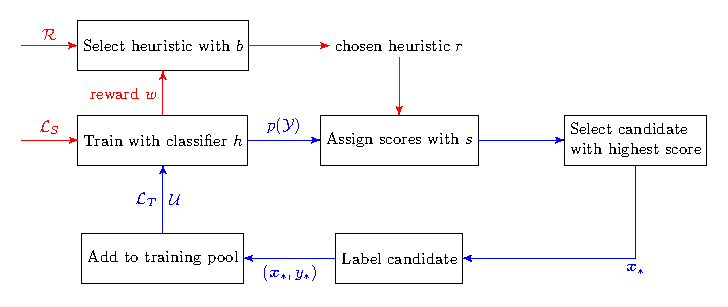
\includegraphics{Fig1}
	\caption{Active learning pipeline with bandit algorithms. We
	need to collect rewards $w$ from the test set $\Labeled_S$ in order to
	decide which heuristic to choose at each time step. This routine is
	indicated by the red arrows. Notations: $\R$ is the set of heuristics
	$\{r_1, ..., r_R\}$, $\Labeled_T$ is the training set, $\Labeled_S$
	is the test set, $\Unlabeled$ is the unlabeled set, and $p(\Y)$ is the
	predicted class probabilities on the unlabeled data $\Unlabeled$.}
	\label{fig:pipeline-bandit}
\end{figure}


\begin{algorithm}[p]
	\KwIn{
    	unlabeled set $\Unlabeled$,
		labeled training set $\Labeled_T$,
		labeled test set $\Labeled_S$,
        classifier $h$,
        desired training size $n$,
        set of active learning heuristics $\R$,
        and bandit algorithm $b$ with two functions \Select\,and \Update.
        }
    \BlankLine
	\While{$|\Labeled_T| < n$}{
		Select a heuristic $r_* \in \R$ according to \Select. \;
		Select the most informative candidate $\bm{x}_*$ from $\Unlabeled$ using the
			chosen heuristic $r_*(\Unlabeled; h)$. \;
        Ask the expert to label $\bm{x}_*$. Call the label $y_*$. \;
		Add the newly labeled example to the training set:
			$\Labeled_T \leftarrow \Labeled_T  \cup \{(\bm{x}_*, y_*)\}$. \;
		Remove the newly labeled example from the unlabeled set:
			$\Unlabeled \leftarrow \Unlabeled \setminus \{ \bm{x}_* \}$. \;
		Retrain the classifier $h(\bm{x})$ using $\Labeled_T$.\;
		Run the updated classifier on the test set $\Labeled_S$ to compute the
			increase in the performance $w$. \;
        Update the parameters of $b$ with \Update$(w)$. \;
    }
	\caption{Pool-based active learning with bandit theory. Note that in
	addition to the set of active learning heuristics $\R$ and the test set
	$\Labeled_S$, some bandit algorithms also need to know $n$, the maximum
	size of the training set, in the advance.}
    \label{alg:bandit}
\end{algorithm}

\subsubsection{Thompson Sampling}

The oldest bandit algorithm is Thompson sampling \citep{thompson33} which
solves the exploration-exploitation trade-off from a Bayesian perspective.

Let $W_i$ be the reward\index{reward} of heuristic $r_i \in \R$. Observe that
even with the best heuristic, we still might not score perfectly due to having
a poor classifier trained on finite data. Conversely, a bad heuristic might be
able to pick an informative candidate due to pure luck. Thus there is always a
certain level of randomness in the reward received. Let us treat the reward
$W_i$ as a normally distributed random variable with mean $\nu_i$ and variance
$\tau_i^2$:
	\begin{align}
		(W_i \mid \nu_i) \sim \Normal(\nu_i, \tau_i^2)
	\end{align}

If we knew both $\nu_i$ and $\tau_i^2$ for all heuristics, the problem would
become trivially easy since we just need to always use the heuristic that has
the highest mean reward. In practice, we do not know the true mean of the
reward $\nu_i$, so let us add a second layer of randomness and assume that
the mean itself follows a normal distribution:
	\begin{align}
        \nu_i \sim \Normal(\mu_i, \sigma_i^2)
    \end{align}

To make the problem tractable, let us assume that the variance $\tau_i^2$ in
the first layer is a known constant. The goal now is to find a good algorithm
that can estimate $\mu_i$ and $\sigma_i^2$.

We start with a prior on $\mu_i$ and $\sigma_i^2$ for each heuristic $r_i$. The
choice of prior does not usually matter in the long run. Since initially we do
not have any information about the performance of each heuristic, the
appropriate prior value for $\mu_i$ is $0$, i.e.\ there is no evidence (yet)
that any of the heuristics offers an improvement to the performance.

In each round, we draw a random sample $\nu_i'$ from the normal distribution
$\Normal(\mu_i, \sigma_i^2)$ for each $i$ and select heuristic $r_*$ that has
the highest sampled value of the mean reward:
    \begin{align}
        r_* = \argmax_{i} \nu_i'
    \end{align}
We then use this heuristic to select the object that is deemed to be the most
informative, add it to the training set, and retrain the classifier. Next we
use the updated classifier to predict the labels of objects in the test set.
Let $w$ be the reward observed. We now have a new piece of information that we
can use to update our prior belief about the mean $\mu_*$ and the variance
$\sigma_*^2$ of the mean reward. Using Bayes' theorem, we can show that the
posterior distribution of the mean reward remains normal,
	\begin{align}
        (\nu_* \mid W_* = w) \sim \Normal (\mu_*', {\sigma'_*}^2)
    \end{align}
with the following new mean and variance:
    \begin{align}
		\mu_*' &= \frac{\mu_* \tau^2_* + w \sigma^2_*}{\sigma^2_* + \tau^2_*}
		&\qquad\qquad
        {\sigma'_*}^2 &= \frac{\sigma^2_* \tau^2_*}{\sigma^2_* + \tau^2_*}
	\end{align}
Algorithm~\ref{alg:thompson} summarizes the \textsc{Select} and \textsc{Update}
functions used in Thompson sampling.
\SetKwFunction{SelectFn}{Select}%
\begin{algorithm}[htbp]
	\Fn{\Select()}{
		\For{$i \in \{1, 2, ..., R\}$}{
			$\nu_i' \leftarrow$ draw a sample from $\Normal(\mu_i, \sigma^2_i)$ \;
			}
		Select the heuristic with the highest sampled value: $r_* \leftarrow \argmax_{i} \nu_i'$ \;
	}
	\BlankLine
	\Fn{\Update($w$)}{
		$\mu_* \leftarrow \dfrac{\mu_* \tau^2_* + w \sigma^2_*}{\sigma^2_* + \tau^2_*}$
		$\qquad\qquad$
		$\sigma_*^2 \leftarrow \dfrac{\sigma^2_* \tau^2_*}{\sigma^2_* + \tau^2_*}$ \;
	}
	\caption{Thompson sampling with normally distributed rewards. Notations:
			$\R$ is the set of $R$ heuristics, $\mu$ is the mean parameter of
			the average reward, $\sigma^2$ is the variance parameter of the
			average reward, $\tau^2$ is the known variance parameter of
			the reward, and $w$ is the actual reward received.}
	\label{alg:thompson}
\end{algorithm}

\subsubsection{Upper Confidence Bounds}

 Next we consider the Upper Confidence Bound (UCB) algorithms which use the
principle of ``optimism in the face of uncertainty''. In choosing which
heuristic to use, we first estimate the upper bound of the reward (that is, we
make an optimistic guess) and pick the one with the highest bound. If our guess
turns out to be wrong, the upper bound of the chosen heuristic will decrease,
making it less likely to get selected in the next iteration.

There are many different algorithms in the UCB family, e.g. UCB1-TUNED \& UCB2
\citep{auer02finite}, V-UCB \citep{audibert09}, OC-UCB \citep{lattimore15}, and
kl-UCB \citep{cappe13}. They differ only in the way the upper bound is
calculated. In this paper, we only consider the last two. In Optimally
Confident UCB (OC-UCB), \cite{lattimore15} suggests that we pick the heuristic
that maximizes the following upper bound:
    \begin{align}
		r_* = \argmax_{i} \Bigg( \overline{w_i} +
			  \sqrt{\dfrac{\alpha}{T_i(t)} \ln\Big(\dfrac{\psi n}{t}\Big)} \Bigg)
    \end{align}
where $\overline{w_i}$ is the average of the rewards from $r_i$ that we have
observed so far, $t$ is the time step, $T_i(t)$ is the number times we have
selected heuristic $r_i$ before step $t$, and $n$ is the maximum number of
steps that we are going to take. There are two tunable parameters, $\alpha$ and
$\psi$, which the author suggests setting to 3 and 2, respectively.

In kl-UCB, \cite{cappe13} suggest that we can instead consider the
KL-divergence between the distribution of the current estimated reward and that
of the upper bound. In the case of normally distributed rewards with known
variance $\sigma^2$, the chosen heuristic would be
    \begin{align}
		r_* = \argmax_{i} \Bigg( \overline{w_i} +
			  \sqrt{ 2 \sigma^2 \dfrac{\ln\big(T_i(t)\big)}{t} } \Bigg)
    \end{align}
Algorithms~\ref{alg:oc-ucb} and~\ref{alg:kl-ucb} summarize these two UCB
approaches. Note that the size of the reward $w$ is not used in
\Update($w$) of UCB, except
to select the best arm.

\begin{algorithm}[htbp]
	\BlankLine
	\Fn{\Select()}{
		$r_* \leftarrow \argmax_{i} \overline{w_i} +
			  \sqrt{\dfrac{3}{T_i(t)} \ln\Big(\dfrac{2 n}{t}\Big)}$ \;
	}
	\BlankLine
	\Fn{\Update($w$)}{
		$t \leftarrow t + 1$ \;
		$T_*(t) \leftarrow T_*(t - 1) + 1$ \;
	}
	\caption{Optimally Confident UCB. Notations:
			 $n$ is the time horizon (maximum number of time steps), $t$ is the
			 current time step, $T_i(t)$ counts of how many times heuristic $i$
			 has been selected before step $t$, $w$ is the reward received, and
			 $\overline{w_i}$ is the average of the rewards from $r_i$ so
			 far.}
	\label{alg:oc-ucb}
\end{algorithm}

\begin{algorithm}[htbp]
	\BlankLine
	\Fn{\Select()}{
		$r_* \leftarrow \argmax_{i} \overline{w_i} +
				\sqrt{2 \sigma^2 \dfrac{\ln\big(T_i(t)\big)}{t}}$ \;
	}
	\BlankLine
	\Fn{\Update($w$)}{
		$t \leftarrow t + 1$ \;
		$T_*(t) \leftarrow T_*(t - 1) + 1$ \;
	}
	\caption{kl-UCB with normally distributed rewards. Notations:
	$\sigma$ is the variance of the rewards, $t$ is the
	current time step, $T_i(t)$ counts of how many times heuristic $i$ has been
	selected before step $t$, $w$ is the reward received, and $\overline{w_i}$ is the
	average of the rewards from $r_i$ so far.}
	\label{alg:kl-ucb}
\end{algorithm}

\subsubsection{EXP3++}

The exponential-weight algorithm for exploration and exploitation (EXP3) was
first developed by \cite{auer2002nonstochastic} to solve the non-stochastic
bandit problem where we make no statistical assumptions about the reward
distribution. This is also often known as the adversarial setting, where we
have an adversary who generates an arbitrary sequence of rewards for each
heuristic in advance. Like Thompson sampling, the algorithm samples from a
probability distribution at each step to pick a heuristic. Here however, we
construct the distribution with exponential weighting (hence the name EXP3). We
shall test~\cite{seldin14}'s EXP3++ algorithm (see Algorithm~\ref{alg:exp3pp}).
This is a generalization of the original EXP3 and it has been shown to perform
well in both the stochastic (where the reward of each heuristic follows an
unknown reward distribution) and the adversarial regime.

\begin{algorithm}[htbp]
	\BlankLine
	\Fn{\Select()}{
		$\beta = \dfrac{1}{2}\sqrt{\dfrac{\ln R}{t R}}$ \;
		\For{$i \in \{1, 2, ..., R\}$}{
			$\xi_i = \dfrac{18 \ln(t)^2}{t \min(1, \dfrac{1}{t} (L_i - \min(L)))^2}$ \;
			$\epsilon_i = \min\large(\dfrac{1}{2 R}, \beta, \xi_i \large)  $ \;
			$\rho_i = \dfrac{e^{-\beta * L_i}}{\sum_j e^{-\beta * L_j}}$ \;
			}
		$r_* \leftarrow \text{draw a sample from $\R$ with
		probability distribution $\rho$}$. \;
	}
	\BlankLine
	\Fn{\Update($w$)}{
		$t \leftarrow t + 1$ \;
		$T_*(t) \leftarrow T_*(t - 1) + 1$ \;
		$L_* \leftarrow \dfrac{L_* + (1 - w)}{(1 - \sum_j \epsilon_j)
			   W_* + \epsilon_*} $
	}
	\caption{EXP3++ algorithm. Notations: $\R$ is the set of $R$ heuristics,
	$t$ is the current time step, $\beta$ is a parameter used to weight the
	heuristics for selection, $\xi_i$ and $\epsilon_i$ are used
	to compute the loss $L_i$, $\rho$ is the distribution from which a heuristic
	is sampled, and $w$ is the reward received.}
	\label{alg:exp3pp}
\end{algorithm}

\subsection{Combining Suggestions with Social Choice Theory}

A drawback of the above bandit methods is that at each iteration, we could only
use one suggestion from one particular heuristic. EXP4 and EXP4.P algorithms
can take advice from all heuristics by maintaining a weight on each of them.
However, being a bandit method, they require designing a reward scheme. If the
reward is the performance on a test set, we would need to keep around a
separate subset of the data, which is expensive and sometimes impossible to
obtain in practice.  This leads us to social choice theory, which can combine
suggestions like EXP4 and EXP4.P, while not needing the concept of a reward.
Originally developed by political scientists like Nicolas de Condorcet and
Jean-Charles de Borda, this field of study is concerned with how we aggregate
preferences of a group of people to determine, for example, the winner in an
election~\citep{list13}. It has the nice property that everyone (or in our
context, every active learning heuristic) has a voice.

For each heuristic, we assign a score to every candidate with the score
function $s(\bm{x}, h)$ like before. We are neither interested in the actual
raw scores nor the candidate with the highest score. Instead, we only need a
ranking of the candidates, which is achieved by a function $k(s, \Unlabeled)$
that provides a ranking of the unlabeled examples according to their scores.
For example, $k$ could assign the candidate with the highest score a rank of 1,
the next best candidate a rank of 2, and so on. An aggregation function $c$
will then combine all the rankings into a combined ranking,
    \begin{align}
		c : \sigma(J_\Unlabeled)^{R} \rightarrow \sigma(J_\Unlabeled)
	\end{align}
where $\sigma(J_\Unlabeled)$ is a permutation over the index set of the
unlabeled pool $\Unlabeled$ and $R$ is the number of heuristics. From these we
can pick the highest-ranked candidate to annotate. See Table~\ref{tab:rank}
for an example.

\begin{table}[htbp]
	\caption {An example of how to convert raw scores into a ranking.}
	          \label{tab:rank}
	\centering
	\begin{tabular}{llllll}
		\toprule
		Score & $s(\bm{x}; h)$  &  0.1 & 0.9 & 0.3 & 0.8 \\
		\midrule
		Rank & $k(s, \Unlabeled)$ & 4 & 1 & 3 & 2 \\
		\bottomrule
	\end{tabular}
\end{table}

The main difference between this approach and the bandit algorithms is that we
do not consider the reward history when combining the rankings. Here each
heuristic is assumed to always have an equal weight. A possible extension,
which is not considered in this paper, is to use the past performance to
re-weight the heuristics before aggregating at each step.
Figure~\ref{fig:pipeline-choice} and Algorithm~\ref{alg:choice} provide an
overview of how social choice theory is used in pool-based active learning.

\begin{figure}[p]
	\centering
	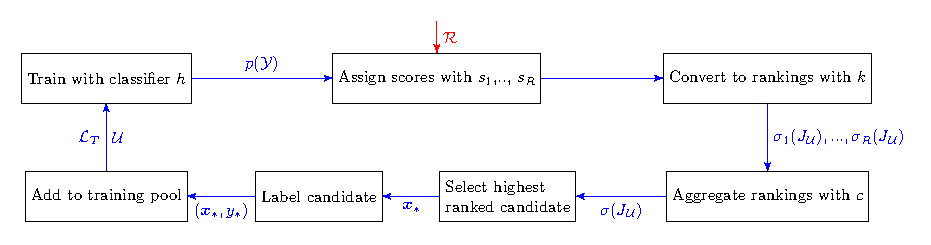
\includegraphics{Fig2}
	\caption{Active learning pipeline with rank aggregation methods. Unlike the
	bandit pipeline, there is only one cycle in which we aggregate information
	from all heuristics. Additional notation: $\sigma(J_\Unlabeled)$ is a
	permutation (i.e. rank) on the index set of the unlabeled data.}
	\label{fig:pipeline-choice}
\end{figure}

\begin{algorithm}[p]
	\KwIn{
    	unlabeled set $\Unlabeled$,
        labeled training set $\Labeled_T$,
        classifier $h$,
		set of active learning suggestions $\R$,
		ranking function $k$,
        and rank aggregator $c$.
        }
    \BlankLine
	\Repeat{we have enough training examples.}{
        \For{$r \in \R$}{
        	Rank all the candidates in $\Unlabeled$ with $k$. \;
        }
        Aggregate all the rankings into one ranking using the aggregator $c$. \;
        Select the highest-ranked candidate $\bm{x}_*$ from $\Unlabeled$. \;
		Ask the expert to label $\bm{x}_*$. Call the label $y_*$. \;
		Add the newly labeled example to the training set:
			$\Labeled_T \leftarrow \Labeled_T  \cup \{(\bm{x}_*, y_*)\}$. \;
		Remove the newly labeled example from the unlabeled set:
			$\Unlabeled \leftarrow \Unlabeled \setminus \{ \bm{x}_* \}$. \;
		Retrain the classifier $h(\bm{x})$ using $\Labeled_T$. \;
    }
    \caption{Pool-based active learning with social choice theory.}
    \label{alg:choice}
\end{algorithm}

The central question in social choice theory is how we can come up with a good
preference aggregation rule. We shall examine three aggregation rules: Borda
count, the geometric mean, and the Schulze method.

In the simplest approach, Borda count, we assign an integer point to each
candidate. The lowest-ranked candidate receives a point of 1, and each
candidate receives one more point than the candidate below. To aggregate, we
simply add up all the points each candidate receives from every heuristic. The
candidate with the most points is declared the winner and is to be labeled
next. We can think of Borda count, then, as ranking the candidate according to
the arithmetic mean.

An alternative approach is to use the geometric mean, where instead of adding
up the points, we multiply them. \cite{bedo14} showed that the geometric mean
maximizes the Spearman correlation between the ranks. Note that this method
requires the ranks to be scaled so that they lie strictly between 0 and 1. This
can be achieved by simply dividing the ranks by $(U + 1)$, where $U$ is the
number of candidates.

The third approach we consider is the Schulze method~\citep{schulze11}. Out of
the three methods considered, this is the only one that fulfills the Condorcet
criterion, i.e. the winner chosen by the algorithm is also the winner when
compared individually with each of the other candidates. However, the Schulze
method is more computationally intensive since it requires examining all pairs
of candidates. First we compute the number of heuristics that prefer candidate
$x_i$ to candidate $x_j$, for all possible pairs $(x_i, x_j)$. Let us call this
$d(x_i, x_j)$. Let us also define a path from candidate $x_i$ to $x_j$ as the
sequence of candidates, $\{ x_i, x_1, x_2,... ,x_j \}$, that starts with $x_i$
and ends with $x_j$, where, as we move along the path, the number of heuristics
that prefer the current candidate over the next candidate must be strictly
decreasing. Intuitively, the path is the rank of a subset of candidates, where
$x_i$ is the highest-ranked candidate and $x_j$ is at the lowest-ranked.

Associated with each path is a strength $p$, which is the minimum of $d(x_i,
x_j)$ for all consecutive $x_i$ and $x_j$ along the path. The core part of the
algorithm involves finding the path of the maximal strength from each
candidate to every other. Let us call $p(x_i, x_j)$ the strength of strongest
path between $x_i$ and $x_j$. Candidate $x_i$ is a potential winner if $p(x_i,
x_j) \geq p(x_j, x_i)$ for all other $x_j$. This problem has a similar flavor
to the problem of finding the shortest path. In fact, the implementation uses a
variant of the Floyd–Warshall algorithm to find the strongest path. This is the
most efficient implementation that we know of, taking cubic time in the number
of candidates.

We end this section with a small illustration of how the three aggregation
algorithms work in Table~\ref{tab:choice}.

\begin{table}[htbp]
	\caption {An example of how social choice theory algorithms rank candidates
	          by aggregating three heuristics: $r_1$, $r_2$, and $r_3$. There
	          are four candidates in the unlabeled pool: A, B, C, and D.}
	          \label{tab:choice}
	\centering
	\begin{subtable}{\linewidth}
		\centering
		\begin{tabular}{lrrrr}
			\toprule
			{Heuristic}  &  Ranking \\
			\midrule
				$r_1$ & B A C D \\
				$r_2$ & A C B D \\
				$r_3$ & B D C A \\
			\bottomrule
		\end{tabular}
		\caption{An example of how the three heuristics rank four candidates
		$A, B, C,$ and $D$. For instance, heuristic $r_1$ considers $B$ to
		be the highest rank candidate, followed by $A$, $C$, and $D$.}
	\end{subtable}

	\begin{subtable}{\linewidth}
		\centering
		\begin{tabular}{lrrrr}
			\toprule
			{Candidate}  &  Borda count & Geometric mean \\
			\midrule
				A & $3 + 4 + 1 = 8$ & $3 \times 4 \times 1 = 12$ \\
				B & $4 + 2 + 4 = 10$ & $4 \times 2 \times 4 = 32$ \\
				C & $2 + 3 + 2 = 7$ & $2 \times 3 \times 2 = 12$ \\
				D & $1 + 1 + 3 = 5$ & $1 \times 1 \times 3 = 3$ \\
			\bottomrule
		\end{tabular}
		\caption{Aggregated ranking with Borda count and geometric mean. The
		scores are determined by the relative ranking in each heuristic. For
		example, $A$ is ranked second by $r_1$, first by $r_1$, and last by
		$r_3$, thus giving us a score of 3, 4 and 1, respectively. In both
		methods, candidate B receives the highest aggregated score.}
	\end{subtable}

	\begin{subtable}{\linewidth}
		\centering
		\begin{tabular}{lrrrr}
			\toprule
			{From / To}  & A & B & C & D \\
			\midrule
				A & -- & 1 & 2 & 2 \\
				B & 2 & -- & 2 & 3 \\
				C & 1 & 1 & -- & 2 \\
				D & 2 & 0 & 1 & -- \\
			\bottomrule
		\end{tabular}
		\caption{Aggregated ranking with the Schulze method. The table shows
		the strongest path strength $p(x_i, x_j)$ between all pairs of
		candidates. For example, $p(B, D) = 3$ because the path $B \rightarrow
		D$ is the strongest path from $B$ to $D$, where three heuristics prefer
		B over D. Candidate B is the winner since $p(B, A) > p(A, B)$, $p(B, C)
		> p(C, B)$, and $p(B, D) > p(D, B)$.}
	\end{subtable}
\end{table}


\section{Experimental Protocol}\label{sec:expt}

We use 11 classification datasets taken from the UCI Machine Learning
Repository\footnote{https://archive.ics.uci.edu/ml/} \citep{lichman13},
with a large multiclass classification dataset which we extracted from the SDSS
project\footnote{https://doi.org/10.5281/zenodo.58500} \citep{alam15}. The
code for the experiments can be found on our GitHub
repository\footnote{https://github.com/chengsoonong/mclass-sky}.
Table~\ref{tab:datasets} shows the size and the number of classes in each
dataset, along with the proportion of the samples belonging to the majority
class and the maximum achievable performance using logistic regression. These
datasets were chosen such that we have an equal number of binary and multiclass
datasets, and a mixture of small and large datasets.

\begin{table}[htbp]

	\caption {Overview of datasets. The following datasets are from the UCI
	Machine Learning Repository: glass, ionosphere, iris, magic, miniboone,
	pageblock, pima, sonar, vehicle, wine, and wpbc. In particular, the vehicle
	dataset comes from the Turing Institute, Glasgow, Scotland. The sdss
	dataset was extracted from Data Release 12 of SDSS-III.}
	\label{tab:datasets}

	\centering
	\begin{tabular}{lrrrrr}
		\toprule
		{Dataset}  & Size &  No. of   & No. of    & Majority & Max Performance  \\
		           &      &  Classes  & Features  &    Class & (MPBA) \\
		\midrule
        \href{https://archive.ics.uci.edu/ml/datasets/Glass+Identification}{glass}
        	& $214$ & $6$ & $10$ & $33\%$ & $65\%$ \\
		\href{https://archive.ics.uci.edu/ml/datasets/Ionosphere}{ionosphere}
			& $351$ & $2$ & $34$ & $64\%$ & $89\%$ \\
		\href{https://archive.ics.uci.edu/ml/datasets/Iris}{iris}
        	& $150$ & $3$ & $4$ & $33\%$ & $90\%$ \\
        \href{https://archive.ics.uci.edu/ml/datasets/MAGIC+Gamma+Telescope}{magic}
        	& $19~020$ & $2$ & $11$ & $65\%$ & $84\%$ \\
        \href{https://archive.ics.uci.edu/ml/datasets/MiniBooNE+particle+identification}{miniboone}
        	& $129~596$ & $2$ & $50$ & $72\%$ & $88\%$ \\
        \href{https://archive.ics.uci.edu/ml/datasets/Page+Blocks+Classification}{pageblock}
        	& $5~473$ & $5$ & $10$ & $90\%$ & $79\%$ \\
		\href{https://archive.ics.uci.edu/ml/datasets/Pima+Indians+Diabetes}{pima}
        	& $733$ & $2$ & $8$ & $66\%$ & $71\%$ \\
        \href{https://doi.org/10.5281/zenodo.58500}{sdss}
        	& $2~801~002$ & $3$ & $11$ & $61\%$ & $90\%$ \\
		\href{https://archive.ics.uci.edu/ml/datasets/Connectionist+Bench+(Sonar,+Mines+vs.+Rocks)}{sonar}
        	& $208$ & $2$ & $60$ & $53\%$ & $78\%$ \\
        \href{https://archive.ics.uci.edu/ml/datasets/Statlog+(Vehicle+Silhouettes)}{vehicle}
			& $846$ & $4$ & $18$ & $26\%$ & $81\%$ \\
		\href{https://archive.ics.uci.edu/ml/datasets/Wine}{wine}
        	& $178$ & $3$ & $13$ & $40\%$ & $94\%$ \\
		\href{https://archive.ics.uci.edu/ml/datasets/Breast+Cancer+Wisconsin+(Prognostic)}{wpbc}
        	& $194$ & $2$ & $34$ & $76\%$ & $58\%$ \\
		\bottomrule
	\end{tabular}
\end{table}

For each dataset, we use Scikit-learn \citep{pedregosa11} to train a logistic
regression model using a 10-fold stratified shuffled cross-validation.
Here `stratified' means that the proportion of the classes remains constant in each
split. We standardize all features to have zero mean and unit variance.
Although all examples have already been labeled, we simulate the active
learning task by assuming that certain examples do not have any labels. For
each fold, the unlabeled pool size is 70\% of data up to a maximum of 10,000
examples, and the test pool consists of the remaining examples up to a maximum
of 20,000. We assume all test examples are labeled. We initialize the
classifier by labeling 10 random instances and using them as the initial
training set. The heuristics are fast enough such that we can assign a score to
every unlabeled instance at every time step. We use logistic regression with a
Gaussian kernel approximation and an L2 regularizer. In the binary case, the
loss function is
\begin{align}
	L &= \dfrac{1}{2} \bm{\theta}^T \bm{\theta} + C \sum_{i = 1}^n
	      \ln\Big(1 + \exp(-y_i(\bm{\theta}^T f(\bm{x}_i)))\Big)
\end{align}
where $\bm{x}_i$ is the feature vector of the $i$th example, $y_i \in \{0, 1\}$
is the label of $\bm{x}_i$, and $n$ is the training size. The term
$\dfrac{1}{2} \bm{\theta}^T \bm{\theta}$ is the regularization term to ensure
that the weight vector $\bm{\theta}$ is not too large, and $C$ is a
regularization hyperparameter in $[10^{-6}, 10^6]$ which we find using grid
search. To speed up the training time while using the Gaussian kernel, we
approximate the feature map of the kernel with Random Kitchen Sinks
\citep{rahimi08}, transforming the raw features $\bm{x}_i$ into a fixed
100-dimensional feature vector $f(\bm{x}_i)$. In the multiclass case, we use
the One-vs-Rest strategy, where for every class we build a binary classifier
that determines whether a particular example belongs to that class or not. For
the QBB algorithms, we train a committee of 7 classifiers, where each member is
given a sample of maximum 100 examples that have already been labeled.

For the bandit algorithms, we use the increase in the mean posterior balanced
accuracy (MPBA) on the test set as the reward. The MPBA can be thought of as
the expected value of the average recall, where we treat the recall as a random
variable that follows a Beta distribution. Compared to the raw accuracy score,
this metric takes into account class imbalance. This is because we first
calculate the recall in each class and then take the average, thus giving each
class an equal weight. Refer to Appendix A for the derivation of the MPBA,
which extends \cite{brodersen10}'s formula from the binary to the multiclass
setting.

In total, we test 17 query strategies. This includes passive learning, 8 active
learning heuristics, 5 bandit algorithms, and 3 aggregation methods. The bandit
algorithms include the four described in Section~\ref{subsec:bandit} and a
baseline called \textsc{explore} which simply selects a random heuristic at
each time step. In other words, we ignore the rewards and explore 100\% of the
time. For all bandit and rank aggregation methods, we take advice from six
representative experts: \textsc{passive}, \textsc{confidence}, \textsc{margin},
\textsc{entropy}, \textsc{qbb-margin}, and \textsc{qbb-kl}. We have not
explored how adding the heuristics with information density weighting to the
bandits would impact the performance. See Table~\ref{tab:abbre} for a list of
abbreviations associated with the methods.
\begin{table}[htbp]
	\caption {Summary of active learning heuristics and combiners used
	in the experiments.} \label{tab:abbre}
	\centering
	\begin{tabular}{lll}
		\toprule
		Abbreviation & Type  & Description \\
		\midrule
        \textsc{passive}
        	& Heuristic & Passive learning \\
		\textsc{confidence}
			& Heuristic & Least confidence heuristic \\
		\textsc{w-confidence}
        	& Heuristic & Least confidence heuristic with information density weighting \\
        \textsc{margin}
        	& Heuristic & Smallest margin heuristic \\
        \textsc{w-margin}
        	& Heuristic & Smallest margin heuristic with information density weighting \\
        \textsc{entropy}
        	& Heuristic & Highest entropy heuristic \\
		\textsc{w-entropy}
        	& Heuristic & Highest entropy heuristic with information density weighting \\
        \textsc{qbb-margin}
        	& Heuristic & Smallest QBB margin heuristic \\
		\textsc{qbb-kl}
        	& Heuristic & Largest QBB KL-divergence heuristic \\
        \textsc{explore}
			& Bandit & Bandit algorithm with 100\% exploration \\
		\textsc{thompson}
        	& Bandit & Thompson sampling \\
		\textsc{ocucb}
			& Bandit & Optimally Confidence UCB algorithm \\
		\textsc{klucb}
			& Bandit & kl-UCB algorithm \\
		\textsc{exp3++}
			& Bandit & EXP3++ algorithm \\
		\textsc{borda}
			& Aggregation & Aggregation with Borda count \\
		\textsc{geometric}
			& Aggregation & Aggregation with the geometric mean \\
		\textsc{schulze}
			& Aggregation & Aggregation with the Schulze method \\
		\bottomrule
	\end{tabular}
\end{table}

Given that there are 12 datasets, each with 17 learning curves, we need a
measure that can summarize in one number how well a particular heuristic or
policy does. Building on~\cite{baram04}'s deficiency measure, we define the
strength of an active learner or a combiner relative to passive learning as
\begin{align}
    \text{Strength}(h; m) &=
    	1 - \dfrac{\sum_{t=1}^{n}\big(m(\max) - m(h, t)\big)}
    	{\sum_{t=1}^{n}\big(m(\max) - m(\passive, t)\big)}
\end{align}
where $m$ is a chosen metric (e.g. accuracy rate, MPBA), $m(\max)$ is the best
possible performance\footnote{The best possible performance in each trial is
obtained by the higher of: 1) the performance achieved by using all the labeled
examples in the training set; and 2) the maximum value of the learning curves
of all the methods.}, and $m(h, t)$ is the performance achieved using the first
$t$ examples selected by heuristic $h$. We can think of the summation as the
area between the best possible performance line and the learning curve of $h$.
The better the heuristic is, the faster it would approach this maximum line,
and thus the smaller the area. Finally, so that we can compare the performance
across datasets, we normalize the measure with the area obtained from using
just passive learning. Refer to Figure~\ref{fig:strength} for a visualization
of the strength measure.

\begin{figure}[htbp]
	\centering
	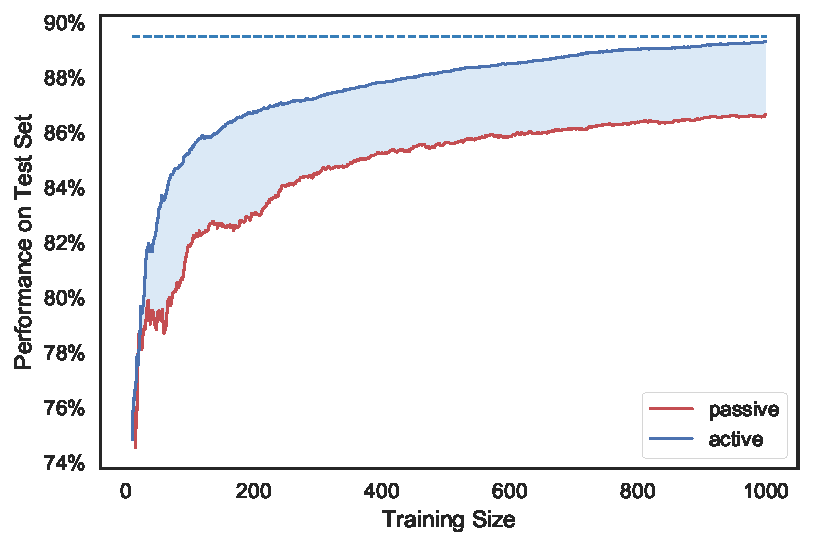
\includegraphics[width=0.7\textwidth]{Fig3}
	\caption[Strength Measure]{An illustration of the MPBA strength measure. It
	is proportional to the shaded area between the (red) passive learning curve
	and the (blue) active learning curve. The bigger the area is, the more the
	active learner outperforms the passive learner. The top dotted line
	indicates the maximum performance achieved.}
	\label{fig:strength}
\end{figure}

We evaluate the algorithm performance with two metrics: the accuracy score and
the MPBA. The accuracy score is the percentage of instances in the test set
where the predicted label matches the true label. If a dataset has a dominant
class, then the accuracy score of instances within that class will also
dominate the overall accuracy score. The MPBA, on the other hand, puts an equal
weight on each class and thus favors algorithms that can predict the label of
all classes equally well.

The heuristics with information density weighting and Thompson sampling have a
few additional hyperparameters. To investigate the effect of these
hyperparameters, we pick one binary dataset (glass) and one multiclass dataset
(ionosphere) to investigate. Both of these are small enough to allow us to
iterate through many hyperparameter values quickly. With \textsc{w-confidence},
\textsc{w-margin}, and \textsc{w-entropy}, we set $\gamma$ in the Gaussian
kernel to be the inverse of the 95\textsuperscript{th} percentile of all
pairwise distances. This appears to work well, as shown in Figure
\ref{fig:gamma}. For \textsc{thompson}, the prior values for $\mu$, $\sigma^2$
and the value of $\tau^2$ seem to have little effect on the final performance
(see Figure \ref{fig:prior}). We set the initial $\mu$ to 0.5, the initial
$\sigma^2$ to 0.02, and $\tau^2$ to 0.02.

\begin{figure}[p]
	\centering
	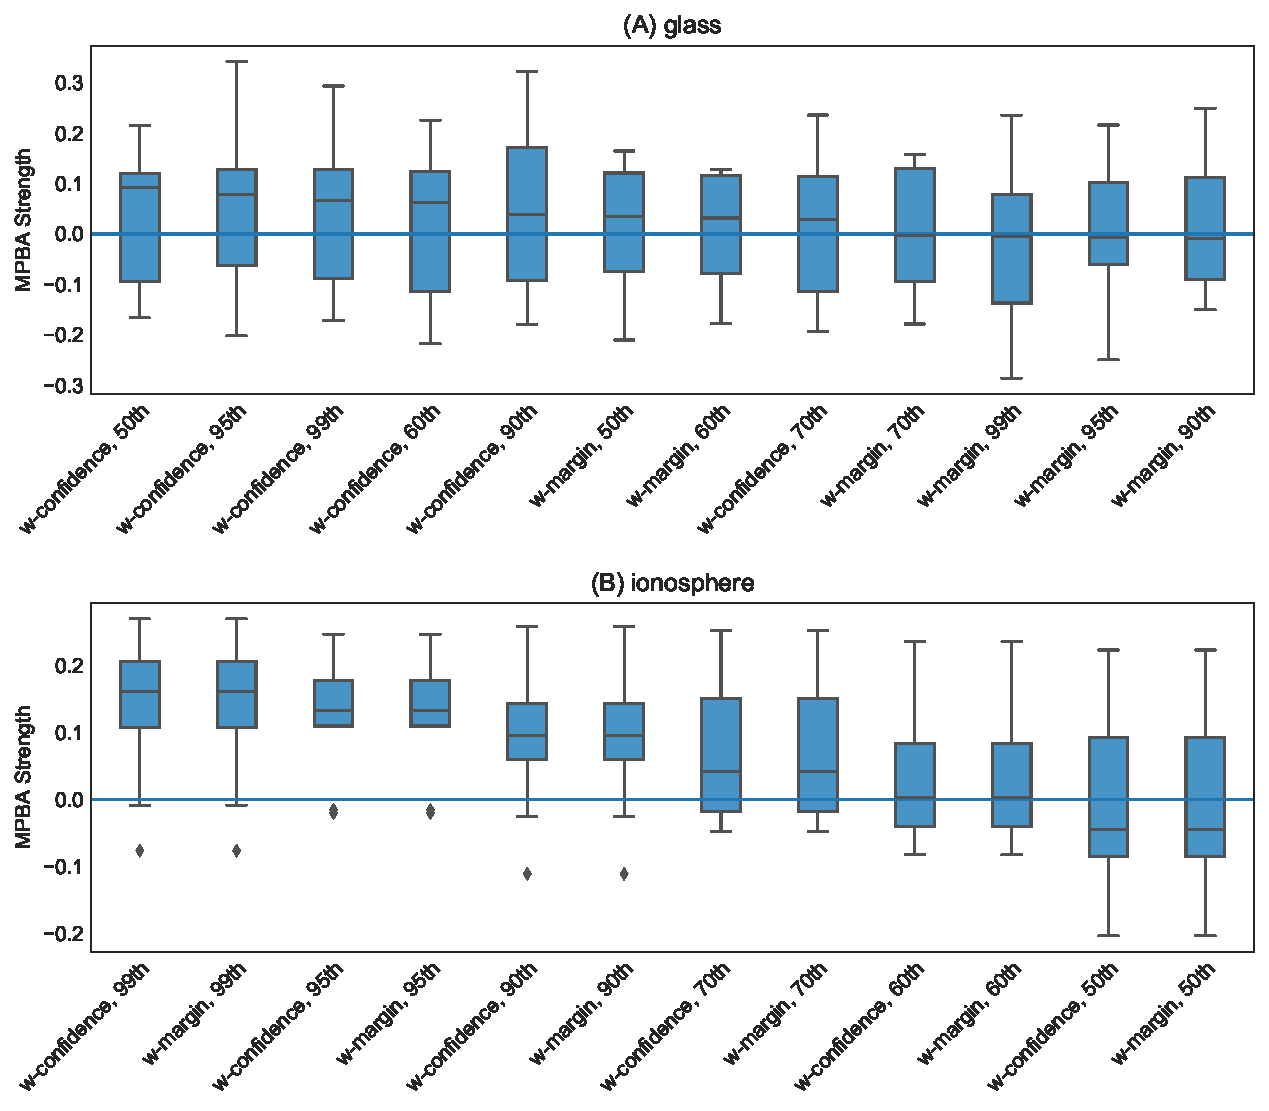
\includegraphics[width=0.7\textwidth]{Fig4}
	\caption[Effect of $\gamma$ in density weighting]{Effect of $\gamma$ on
	\textsc{w-confidence} and \textsc{w-margin} using the glass and ionosphere
	datasets. We examine six different values for $\gamma$: the
	50\textsuperscript{th}, 60\textsuperscript{th}, 70\textsuperscript{th},
	90\textsuperscript{th}, 95\textsuperscript{th}, and 99\textsuperscript{th}
	percentile of the of the pairwise L1-distance between the data points. For
	the glass dataset, changing value of $\gamma$ has minimal effect on the
	results, while for the ionosphere dataset, using the 90\textsuperscript{th}
	percentile and above seems to work well.}
	\label{fig:gamma}
\end{figure}

\begin{figure}[p]
	\centering
	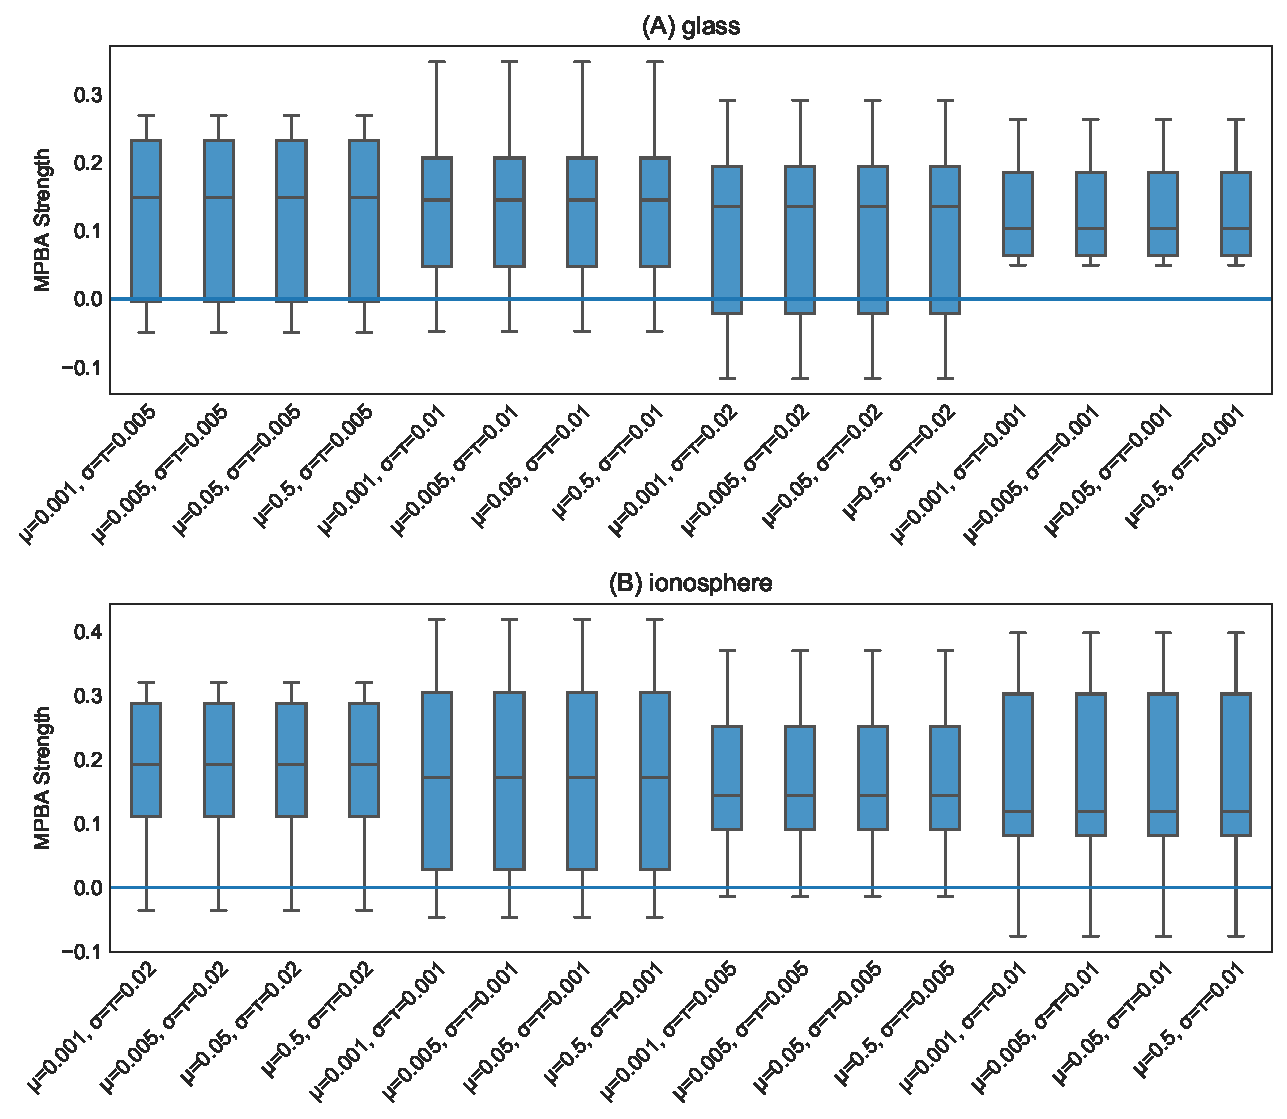
\includegraphics[width=0.7\textwidth]{Fig5}
	\caption[Effect of the parameters on Thompson sampling]{Effect of the
	initial values of the parameters in \textsc{thompson}. We test 16
	combinations of $\mu$, $\sigma^2$, and $\tau^2$ on the glass and ionosphere
	dataset. Varying these values does not seem to affect the final
	performance.}
	\label{fig:prior}
\end{figure}



\section{Results}\label{sec:results}

Figures~\ref{fig:strengths-small} and~\ref{fig:strengths-large} show the
strengths of all methods that we consider, while
Figures~\ref{fig:learning_curves-small} and~\ref{fig:learning_curves-large}
provide selected learning curves. Plots for the 6 small datasets with fewer
than 500 examples (glass, ionosphere, iris, sonar, wine, and wpbc) are shown in
Figures~\ref{fig:strengths-small} and Figure~\ref{fig:learning_curves-small}.
Plots for the 2 medium-sized datasets (pima and vehicle) and the 4 large
datasets (magic, miniboone, pageblocks, and sdss) are shown in
Figure~\ref{fig:strengths-large} and Figure~\ref{fig:learning_curves-large}.
Each figure contains two subfigures, one reporting the raw accuracy score,
while the other showing the MPBA score.

Active learning methods generally beat passive learning in four of the six
small datasets---glass, ionosphere, iris, and wine. This can be seen by the
fact that the boxplots are mostly above the zero line in Figure
\ref{fig:strengths-small}. For sonar and wpbc, the results are mixed---active
learning has little to no effect here. The wpbc dataset is particularly
noisy---our classifier cannot achieve an MPBA score greater than 60\% (see
Figure \ref{fig:learning_curves-small}). Thus it is not surprising that active
learning does not perform well here since there is not much to learn to begin
with.

The advantage of active learning becomes more apparent with the larger datasets
like magic, miniboone, pageblocks, and sdss. Here there is a visible gap
between the passive learning curve and the active learning curve for most
methods. For instance, using a simple heuristic such as \textsc{confidence} in
the pageblocks dataset results in an average MPBA score of 74\% after 1,000
examples, while passive learning can only achieves 67\% (see Figure
\ref{fig:learning_curves-large}F).


Out of the 8 active learning heuristics tested, the heuristics with the
information density weighting (\textsc{w-confidence}, \textsc{w-margin}, and
\textsc{w-entropy}) generally perform worse than the ones without the
weighting. \textsc{qbb-kl} performs the best in pageblocks while it can barely
beat passive learning in other datasets. The remaining
heuristics---\textsc{confidence}, \textsc{margin}, \textsc{entropy}, and
\textsc{qbb-margin}---perform equally well in all datasets.

We find no difference in performance between the bandit algorithms and
the rank aggregation methods. Combining active learners does not seem
to hurt the performance, even if we include a poorly performing heuristic
such as \textsc{qbb-kl}.

For bandit algorithms, it is interesting to note that \textsc{thompson} favors
certain heuristics a lot more than others, while the behavior of
\textsc{exp3++}, \textsc{ocucb}, and \textsc{klucb} is almost indistinguishable
from \textsc{explore}, where we explore 100\% of the time (see Figure
\ref{fig:selection}). Changing the initial values of $\mu$, $\sigma^2$, and
$\tau^2$ changes the order of preference slightly, but overall, which
heuristics \textsc{thompson} picks seems to correlate with the heuristic
performance. For example, as shown in Figure
\ref{fig:selection-thompson-params}, \textsc{passive}
and \textsc{qbb-kl} tend to get chosen less often than others in the ionosphere
dataset.


\begin{figure}[tbp]
	\centering
	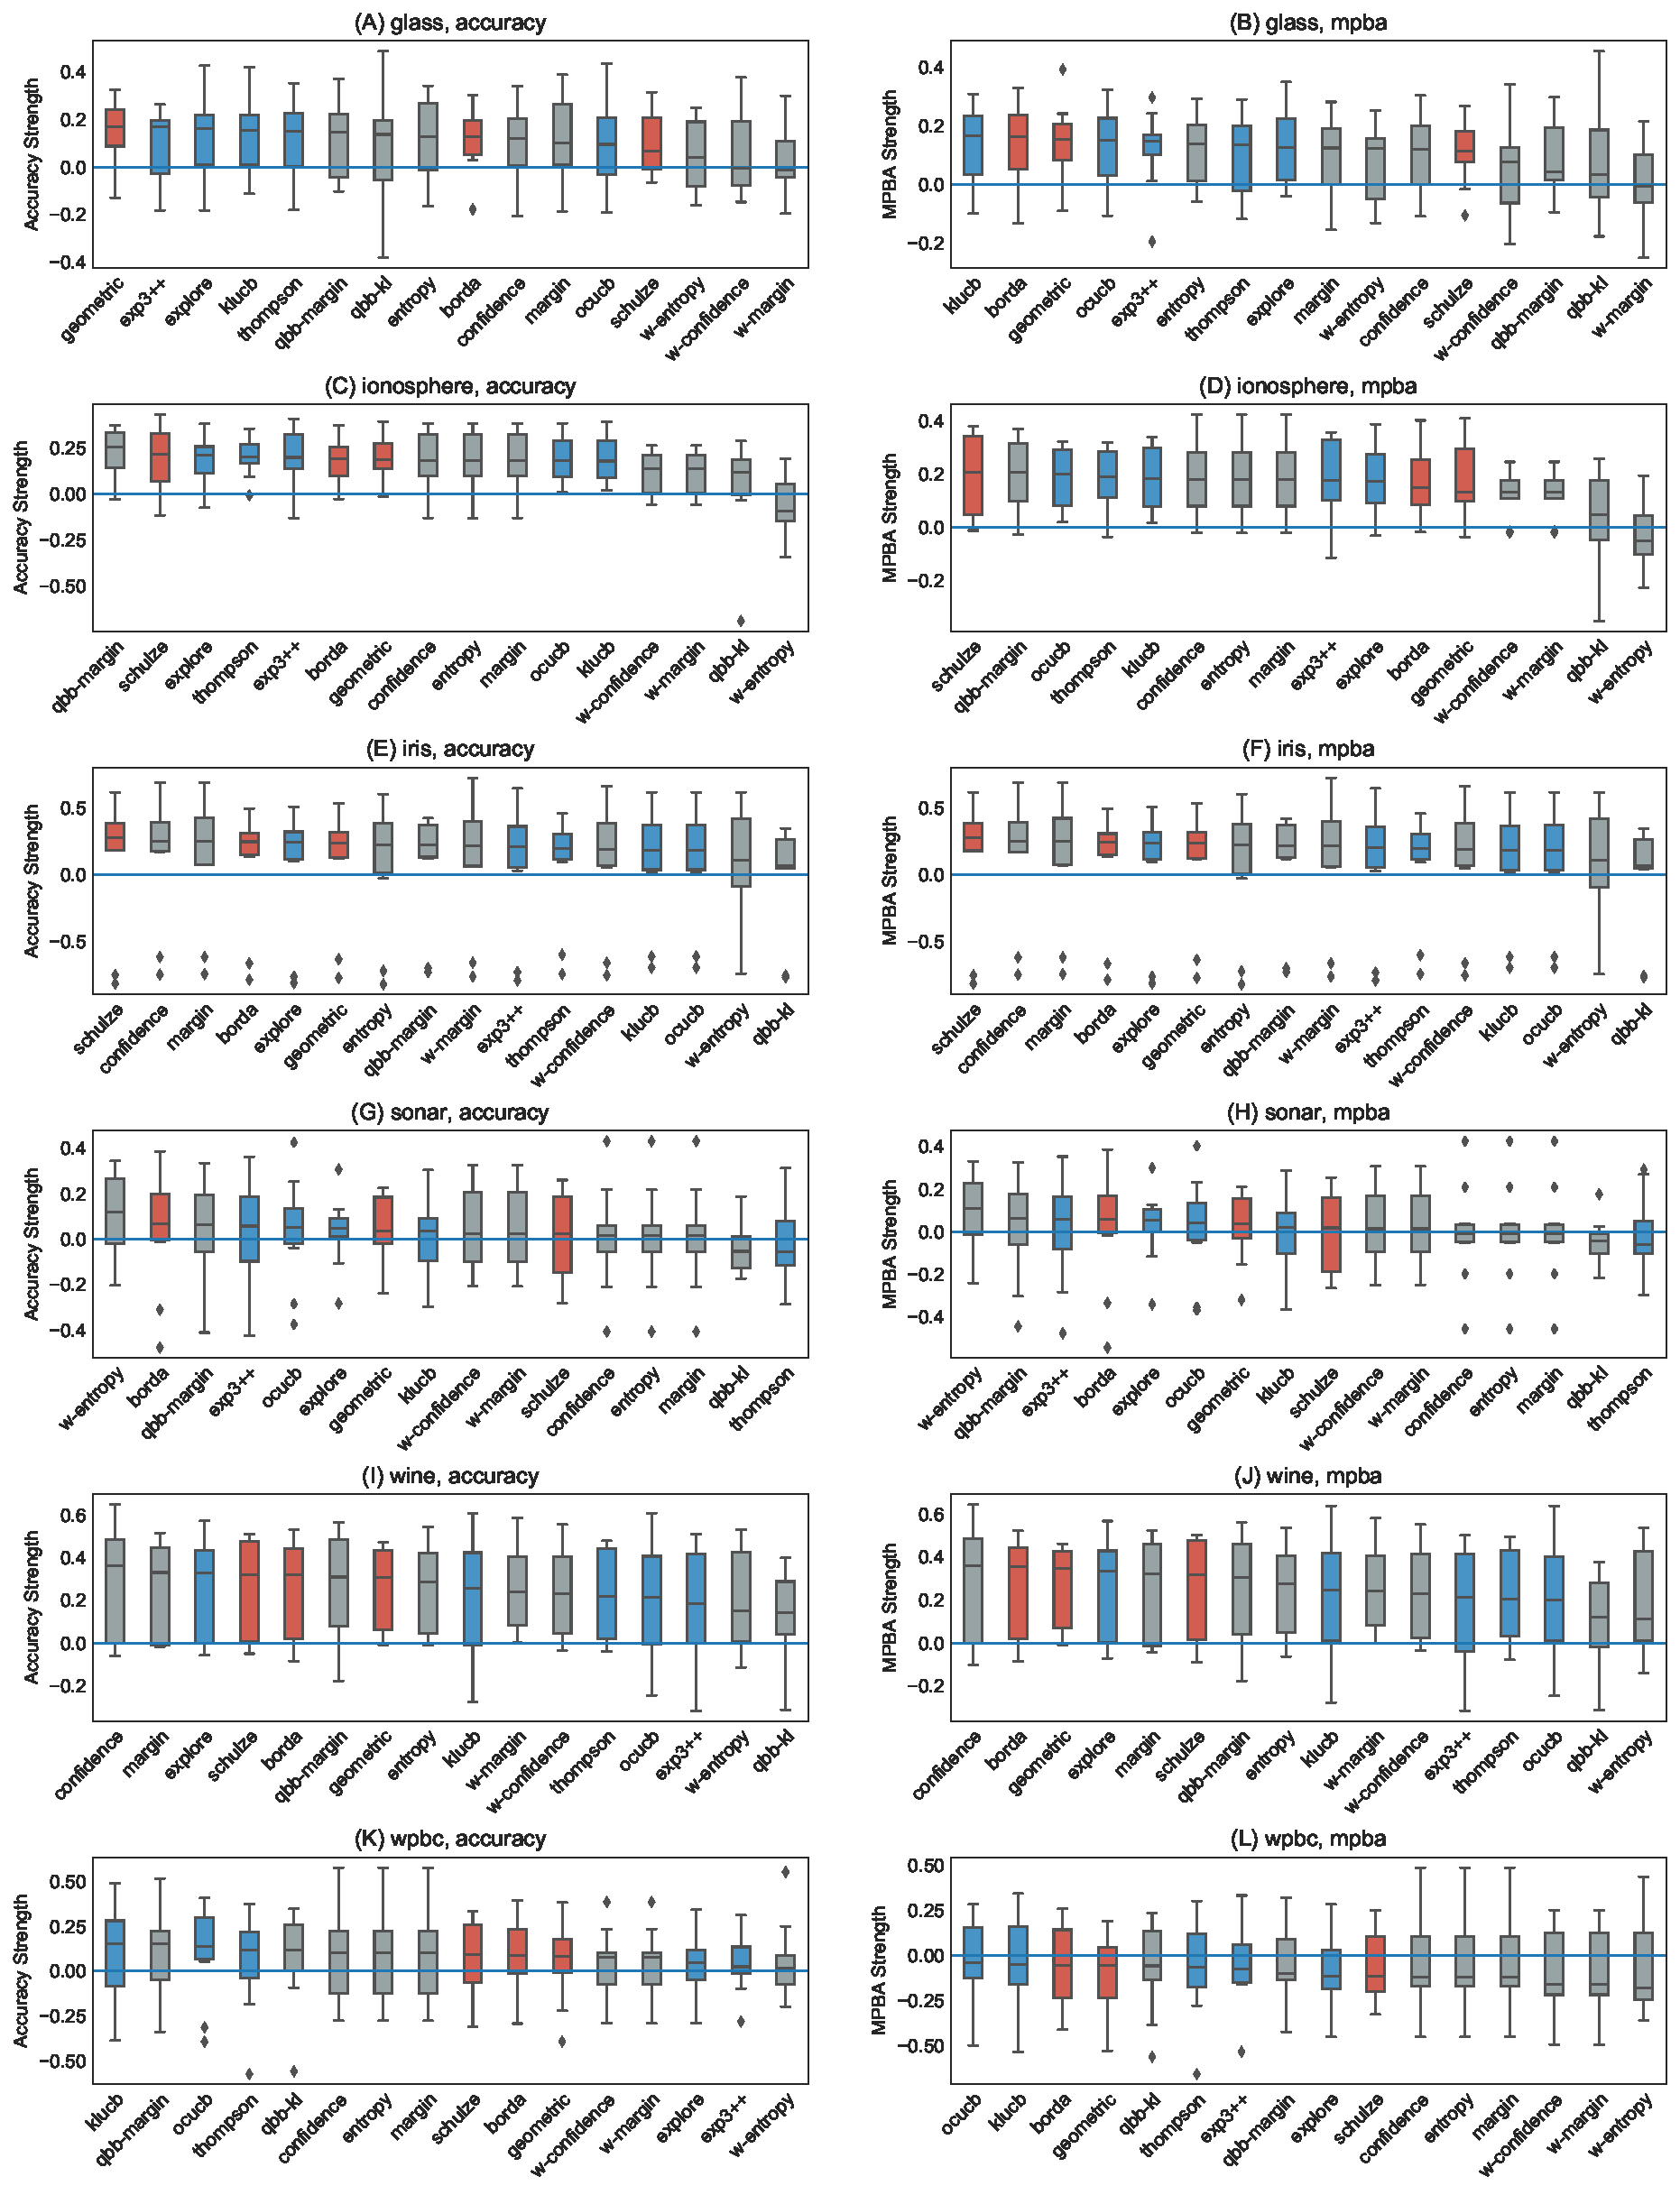
\includegraphics[width=\textwidth]{Fig6}
	\caption[Policy strength]{Boxplots of the accuracy and MPBA strength of the
	16 active learning strategies, relative to passive learning, using the
	small datasets (glass, ionosphere, iris, sonar, wine, and wpbc). The more
	positive the strength is, the better the heuristic/combiner is. Gray boxes
	represent individual heuristics; blue boxes represent bandit algorithms, and
	red boxes are for rank aggregation methods. A strategy that is above the
	zero line is better than passive learning. Each boxplot contains 10 trials.
	The accuracy score is a simple metric that simply counts up the number of
	correct predictions. The MPBA score, being the weighted average of the
	recall and precision, gives an equal representation to each class. The
	boxes represent the quartiles and the whiskers extend to 1.5 times of the
	interquartile range.}
	\label{fig:strengths-small}
\end{figure}

\begin{figure}[tbp]
	\centering
	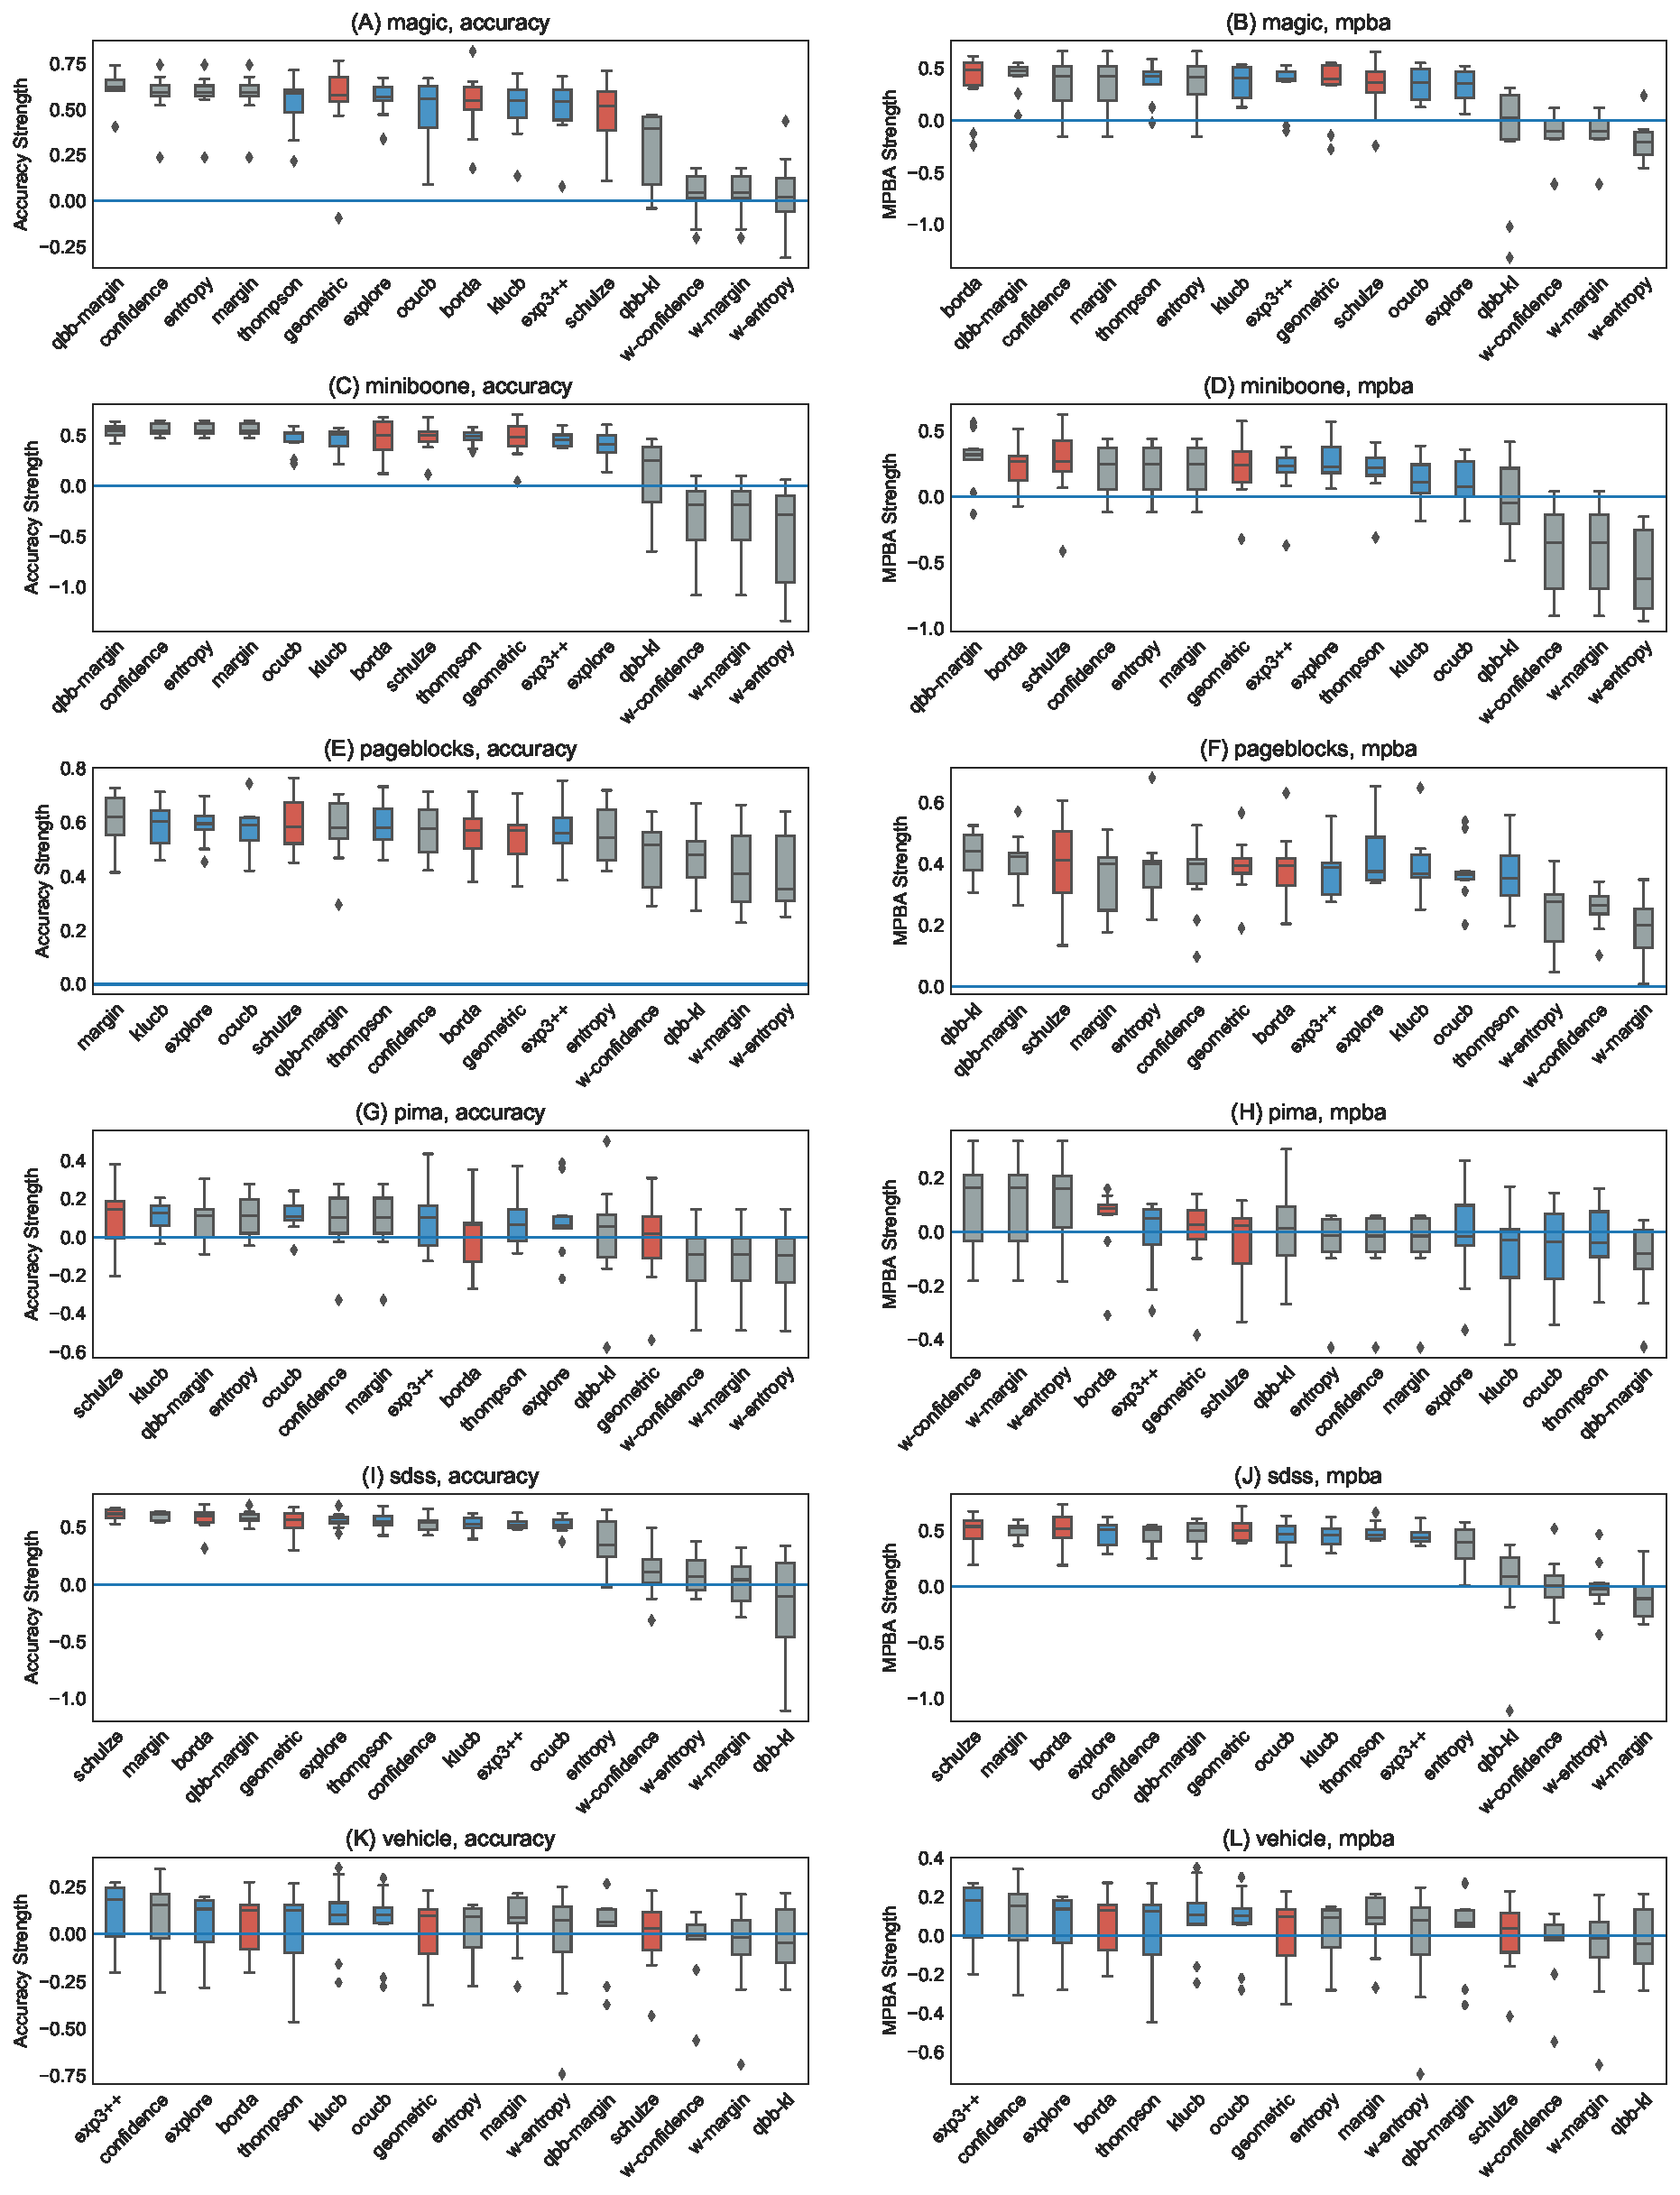
\includegraphics[width=\textwidth]{Fig7}
	\caption[Policy strength]{Boxplots of the accuracy and MPBA strength of the
	16 active learning strategies, relative to passive learning, using medium
	to the large datasets (magic, miniboone, pageblocks, pima, sdss, and
	vehicle). The more positive the strength is, the better the
	heuristic/combiner is. Gray boxes represent individual heuristics; blue
	boxes represent bandit algorithms, and red boxes are for rank aggregation
	methods. A strategy that is above the zero line is better than passive
	learning. Each boxplot contains 10 trials. The accuracy score is a simple
	metric that simply counts up the number of correct predictions. The MPBA
	score, being the weighted average of the recall and precision, gives an
	equal representation to each class. The boxes represent the quartiles and
	the whiskers extend to 1.5 times of the interquartile range.}
	\label{fig:strengths-large}
\end{figure}


\begin{figure}[tbp]
	\centering
	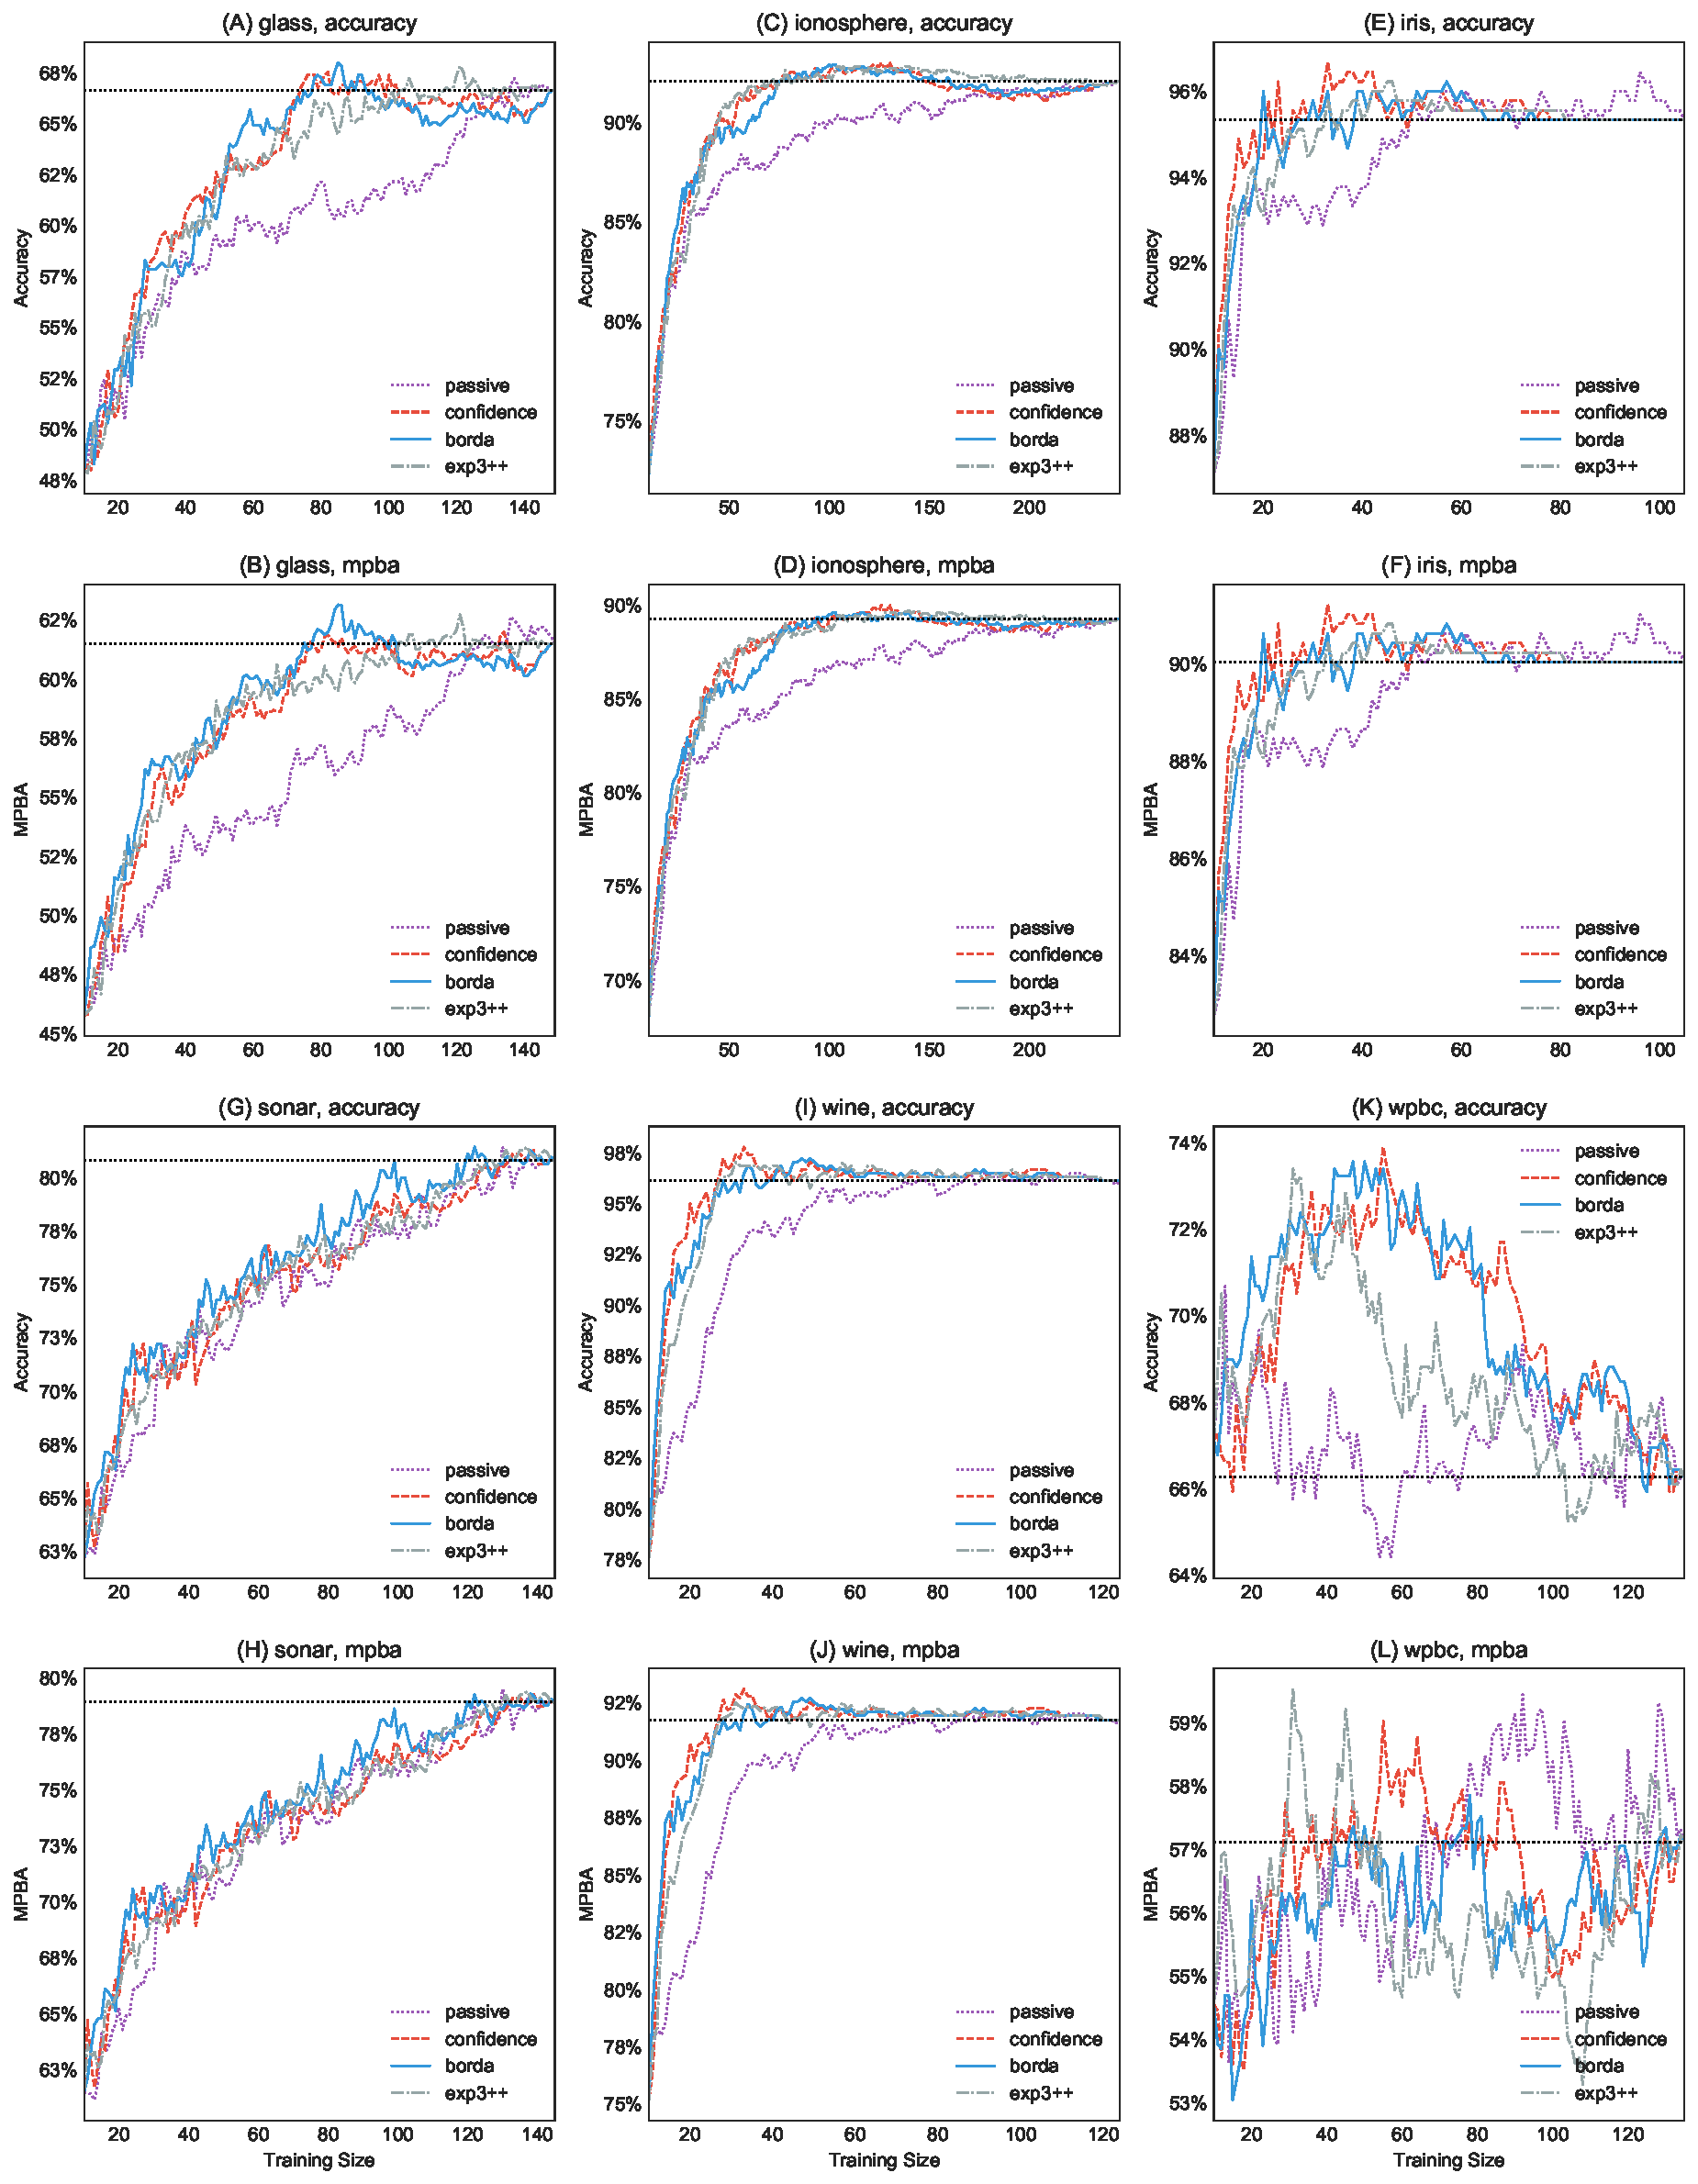
\includegraphics[width=\textwidth]{Fig8}
	\caption[Selected learning curves]{Selected accuracy and MPBA learning
	curves for the small datasets (glass, ionosphere, iris, sonar, wine, and
	wpbc). As it would get too cluttered to plot 17 learning curves, we only
	show the learning curve for \textsc{passive}, \textsc{confidence},
	\textsc{exp3++}, and \textsc{borda}. The learning curves are averaged over
	10 trials. The dotted horizontal line shows the performance obtained from
	using the whole training data.}
	\label{fig:learning_curves-small}
\end{figure}

\begin{figure}[tbp]
	\centering
	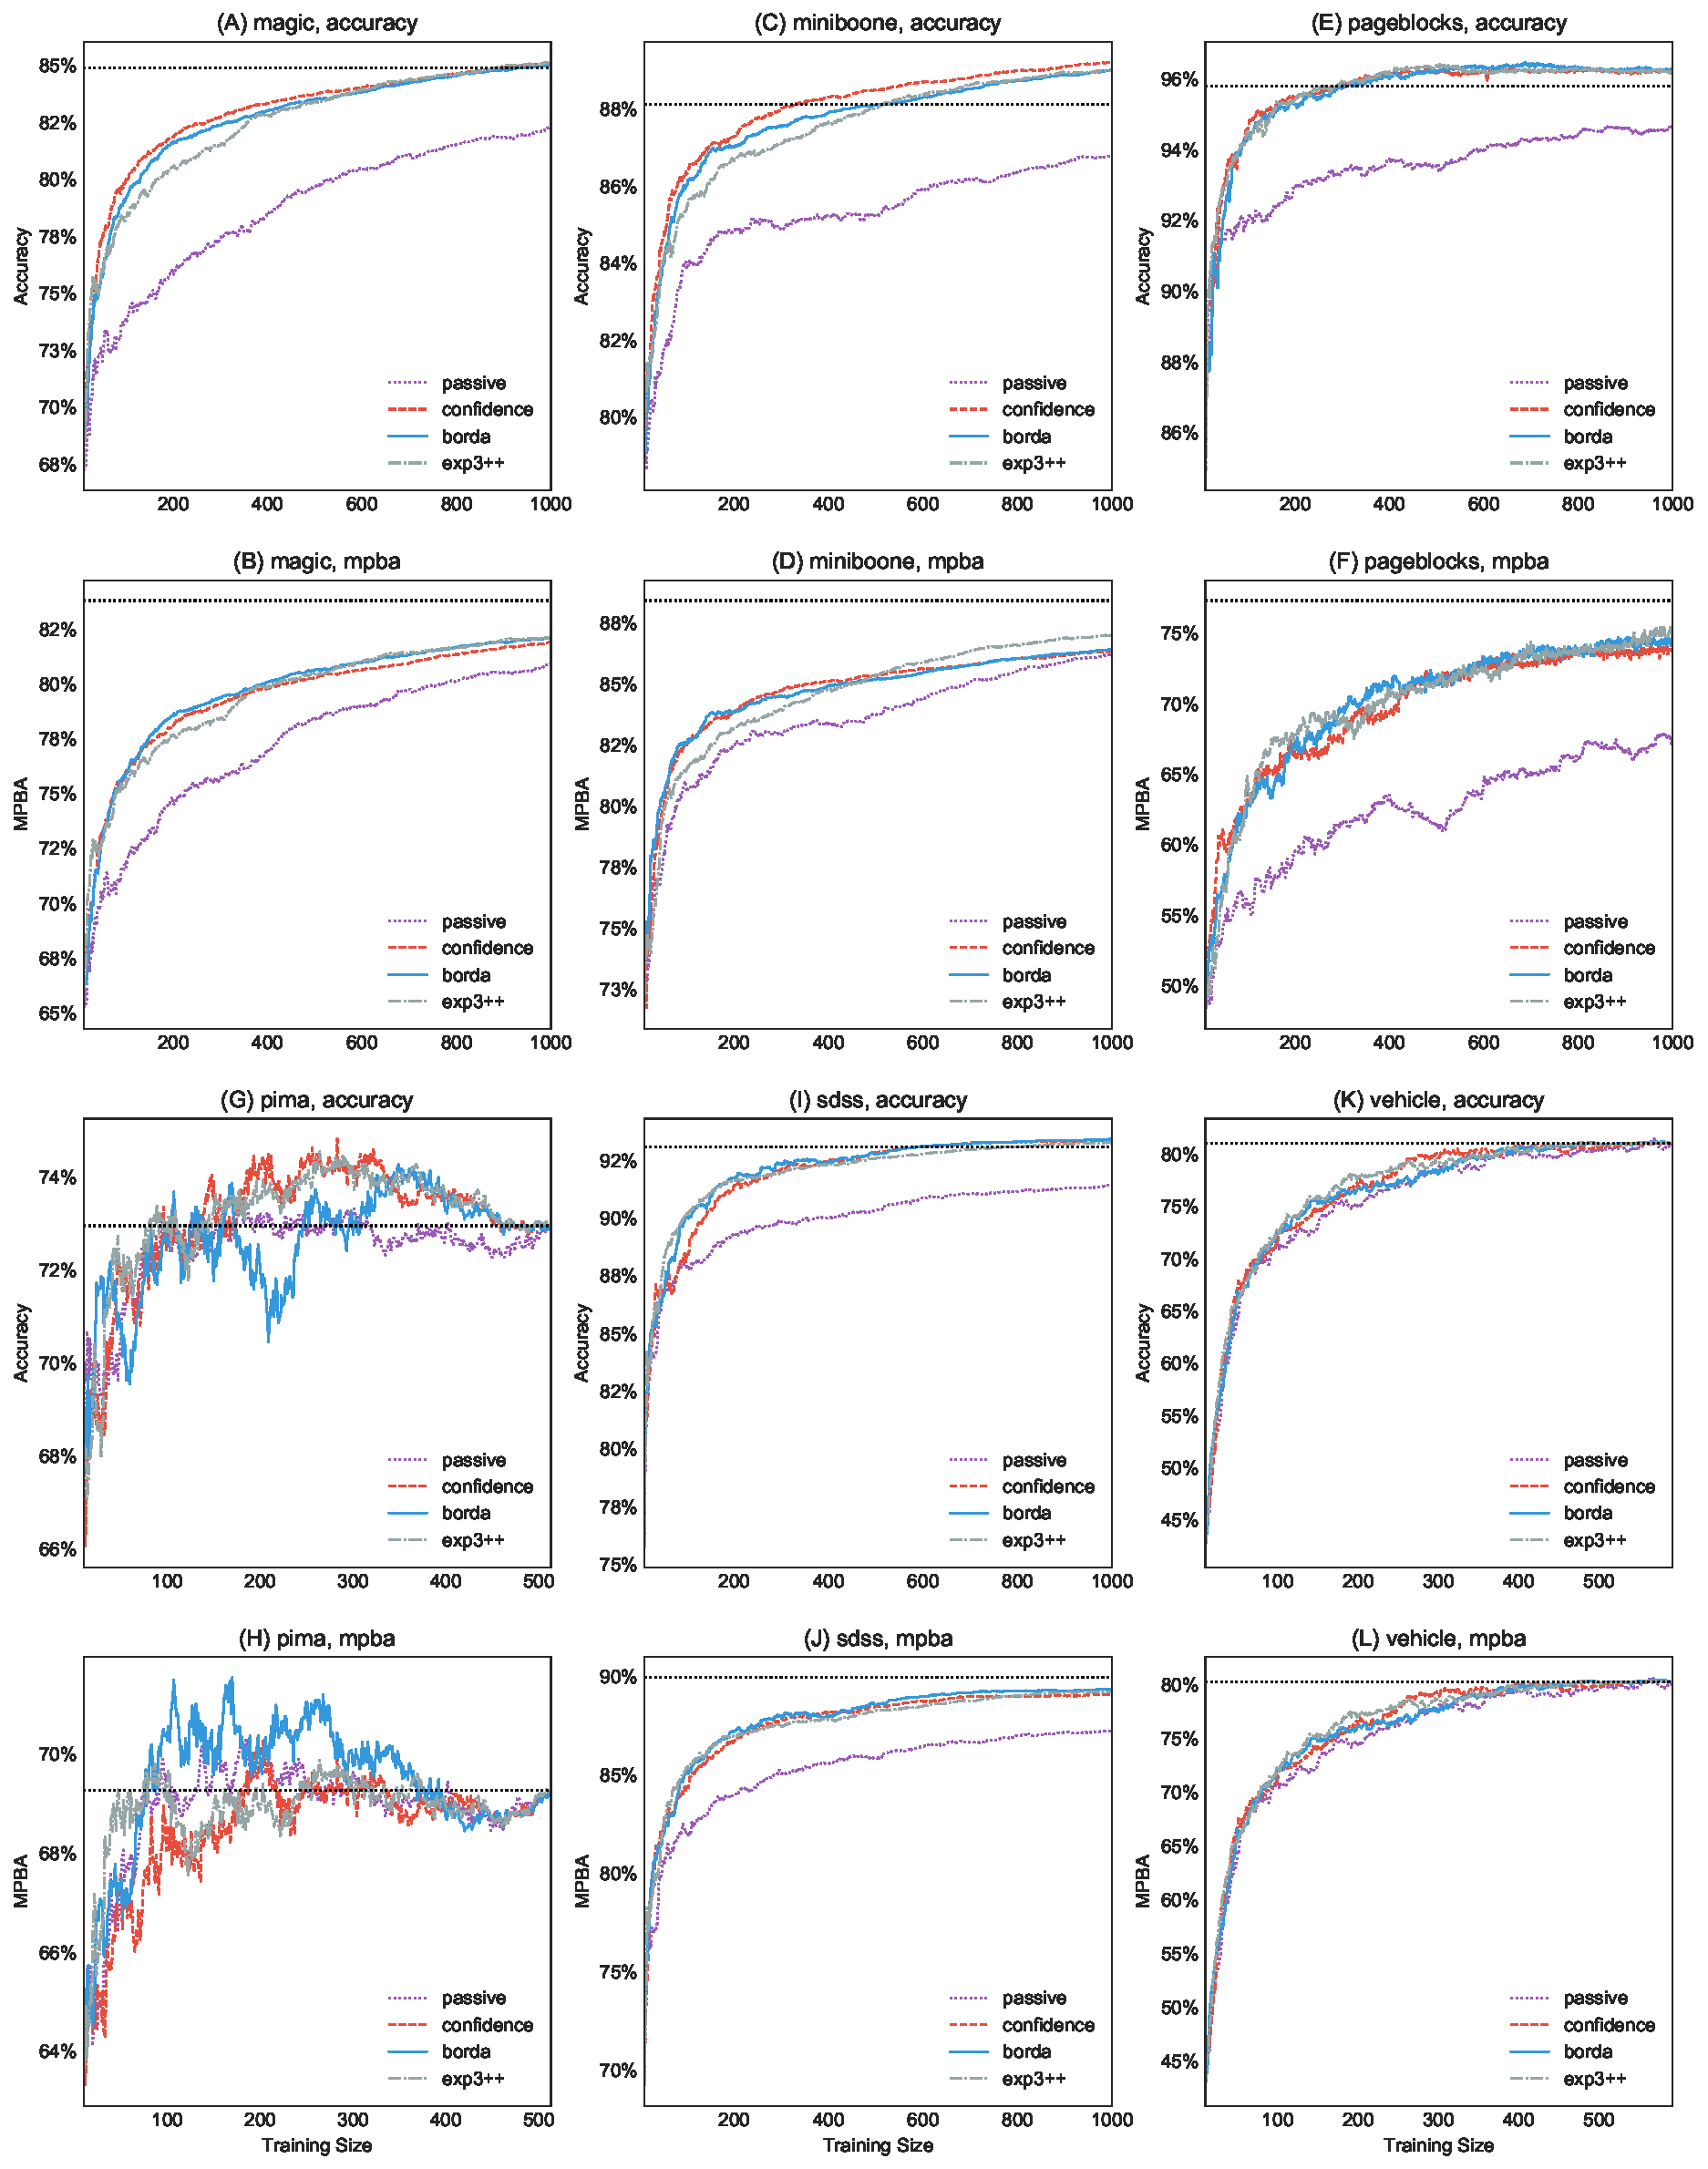
\includegraphics[width=\textwidth]{Fig9}
	\caption[Selected learning curves]{Selected accuracy and MPBA learning
	curves for the medium to large datasets (magic, miniboone, pageblocks,
	pima, sdss, and vehicle). As it would get too cluttered to plot 17 learning
	curves, we only show the learning curve for \textsc{passive},
	\textsc{confidence}, \textsc{exp3++}, and \textsc{borda}. The learning
	curves are averaged over 10 trials. The dotted horizontal line shows the
	performance obtained from using the whole training data.}
	\label{fig:learning_curves-large}
\end{figure}

\begin{figure}[tbp]
	\centering
	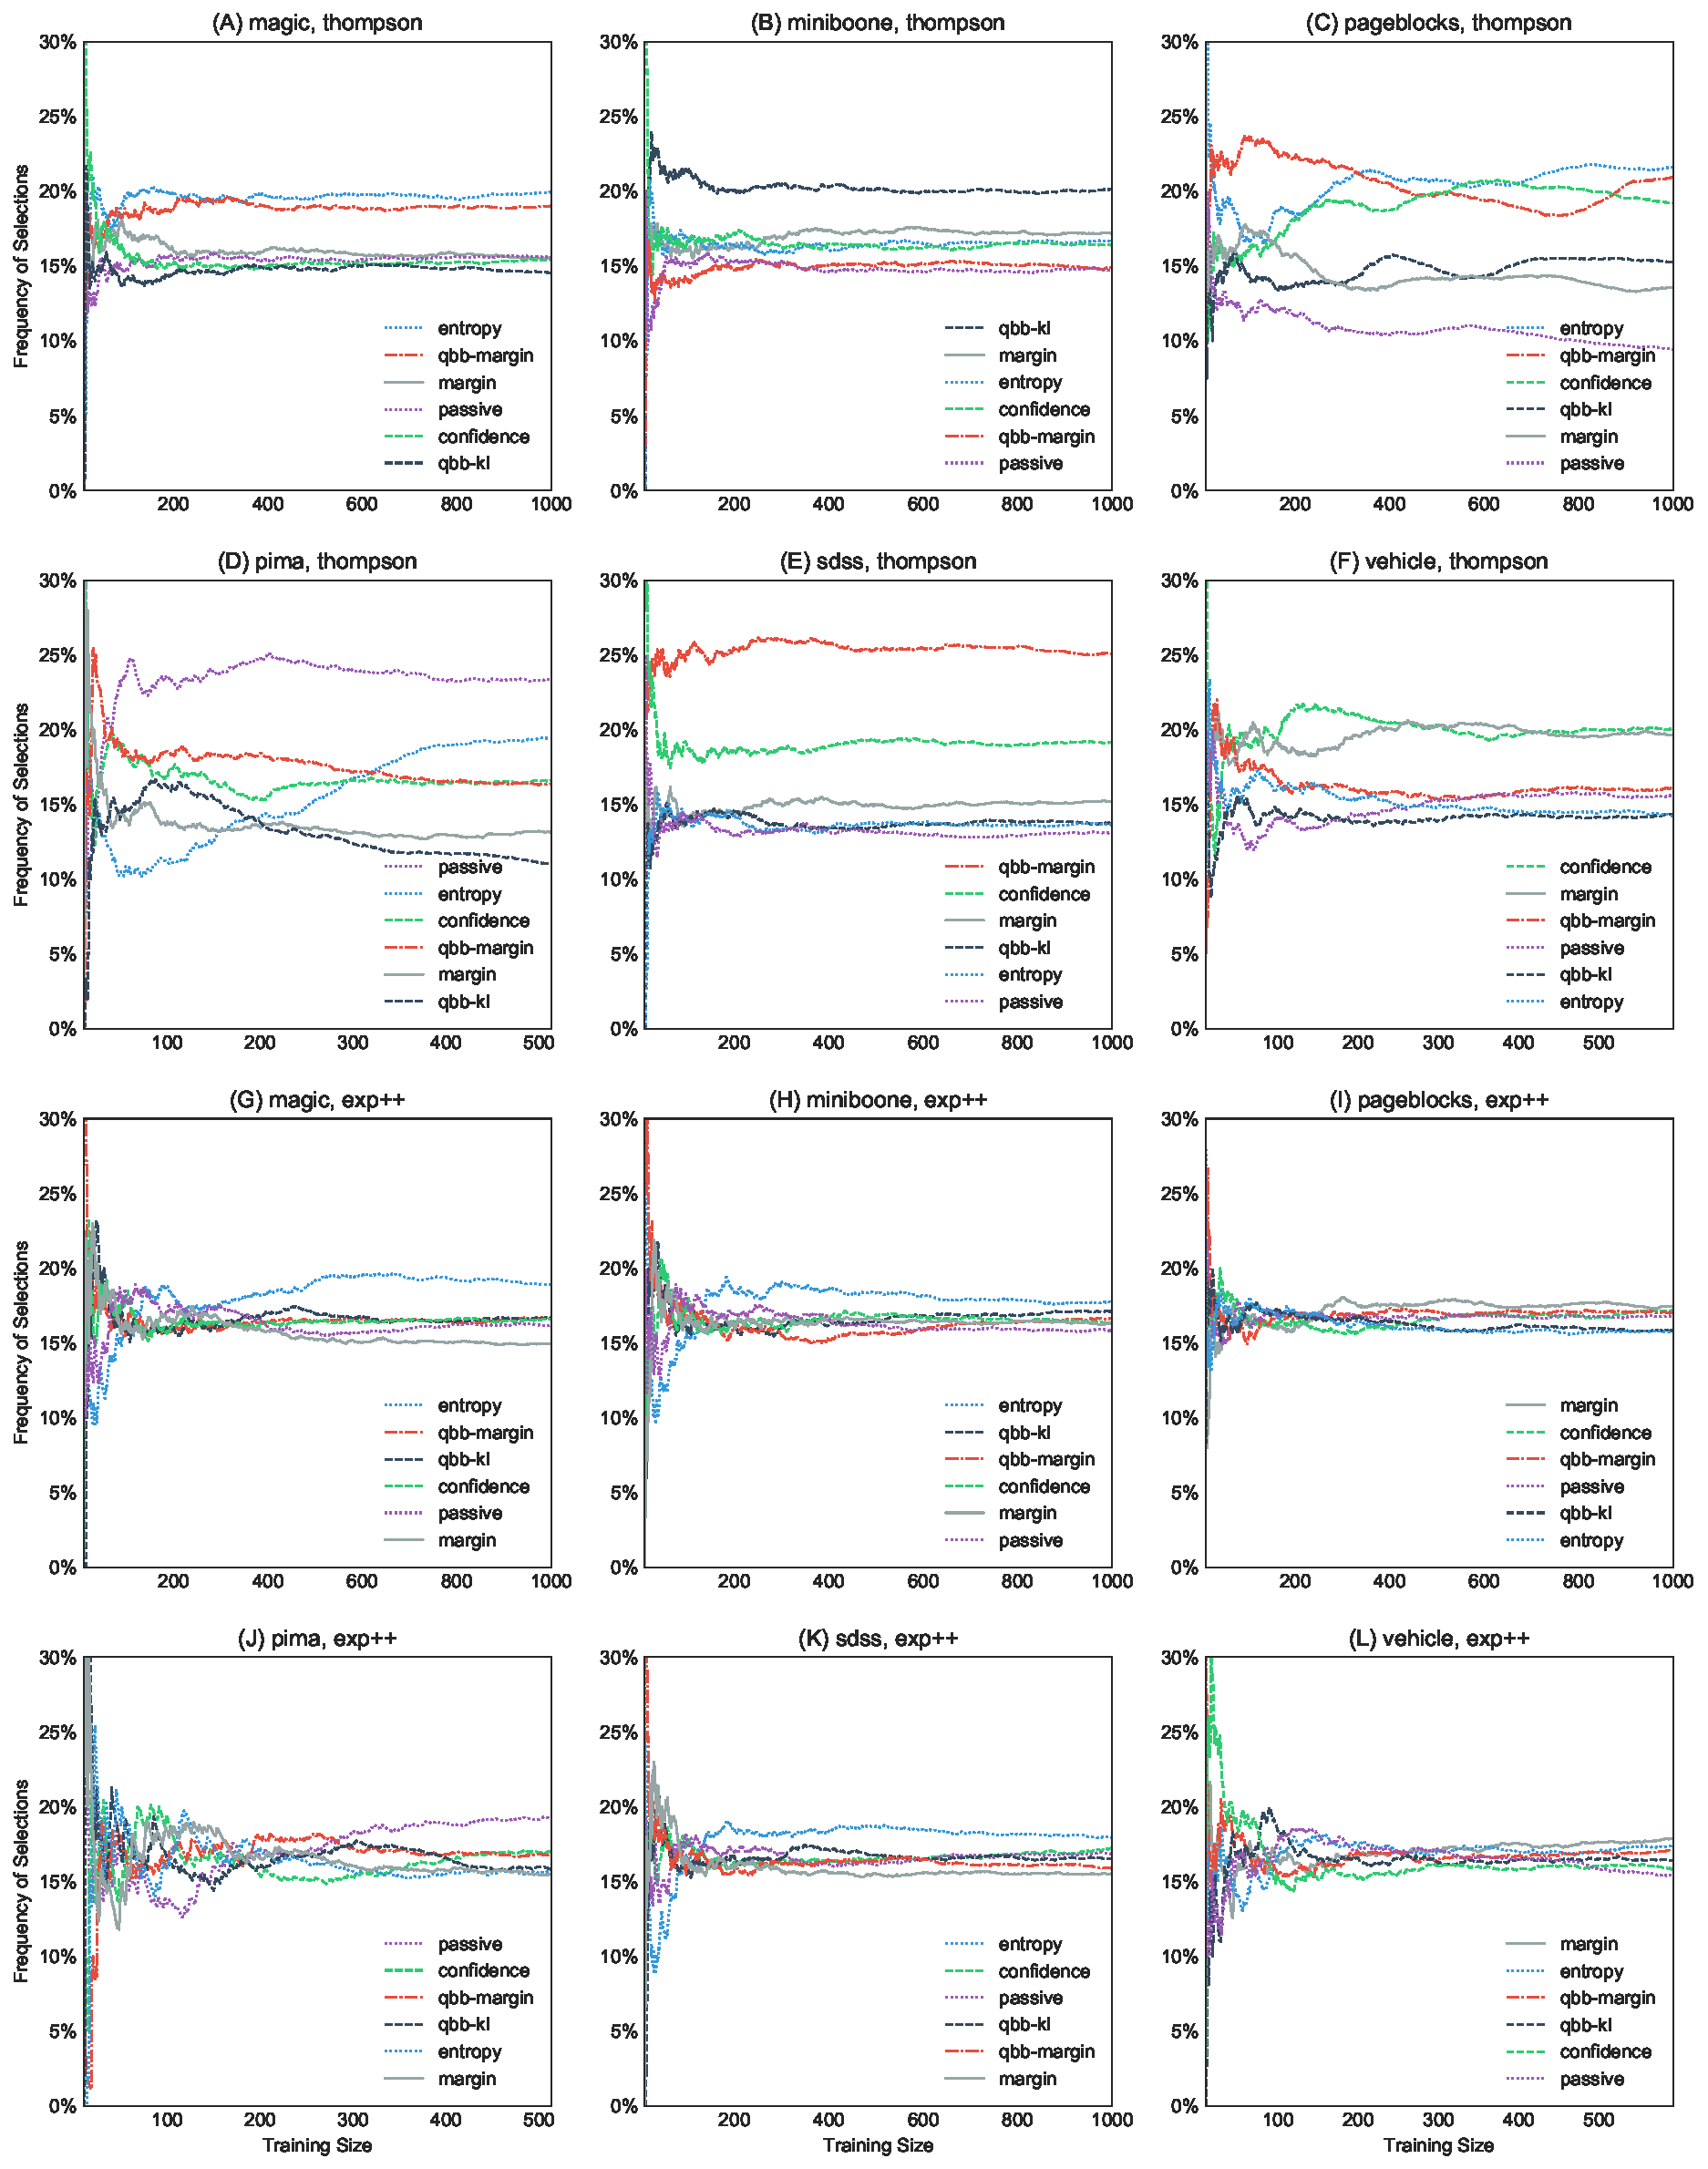
\includegraphics[width=\textwidth]{Fig10}
	\caption[Heuristic selection frequencies]{Selection frequencies of
	heuristics in \textsc{thompson} and \textsc{exp3++}, with the large
	datasets (magic, miniboone, pageblocks, pima, sdss, and vehicle). The plots
	show how often each of the heuristics gets selected over time. The
	selection frequencies are averaged over 10 trials. \textsc{thompson} favors
	certain heuristics more strongly than others. In contrast, \textsc{exp3++}
	favors uniform exploration more, sampling each heuristic with roughly equal
	weights. The plots for \textsc{ocucb} and \textsc{klucb} are not shown
	here, but they are similar to \textsc{exp3++}.}
	\label{fig:selection}
\end{figure}

\begin{figure}[tbp]
	\centering
	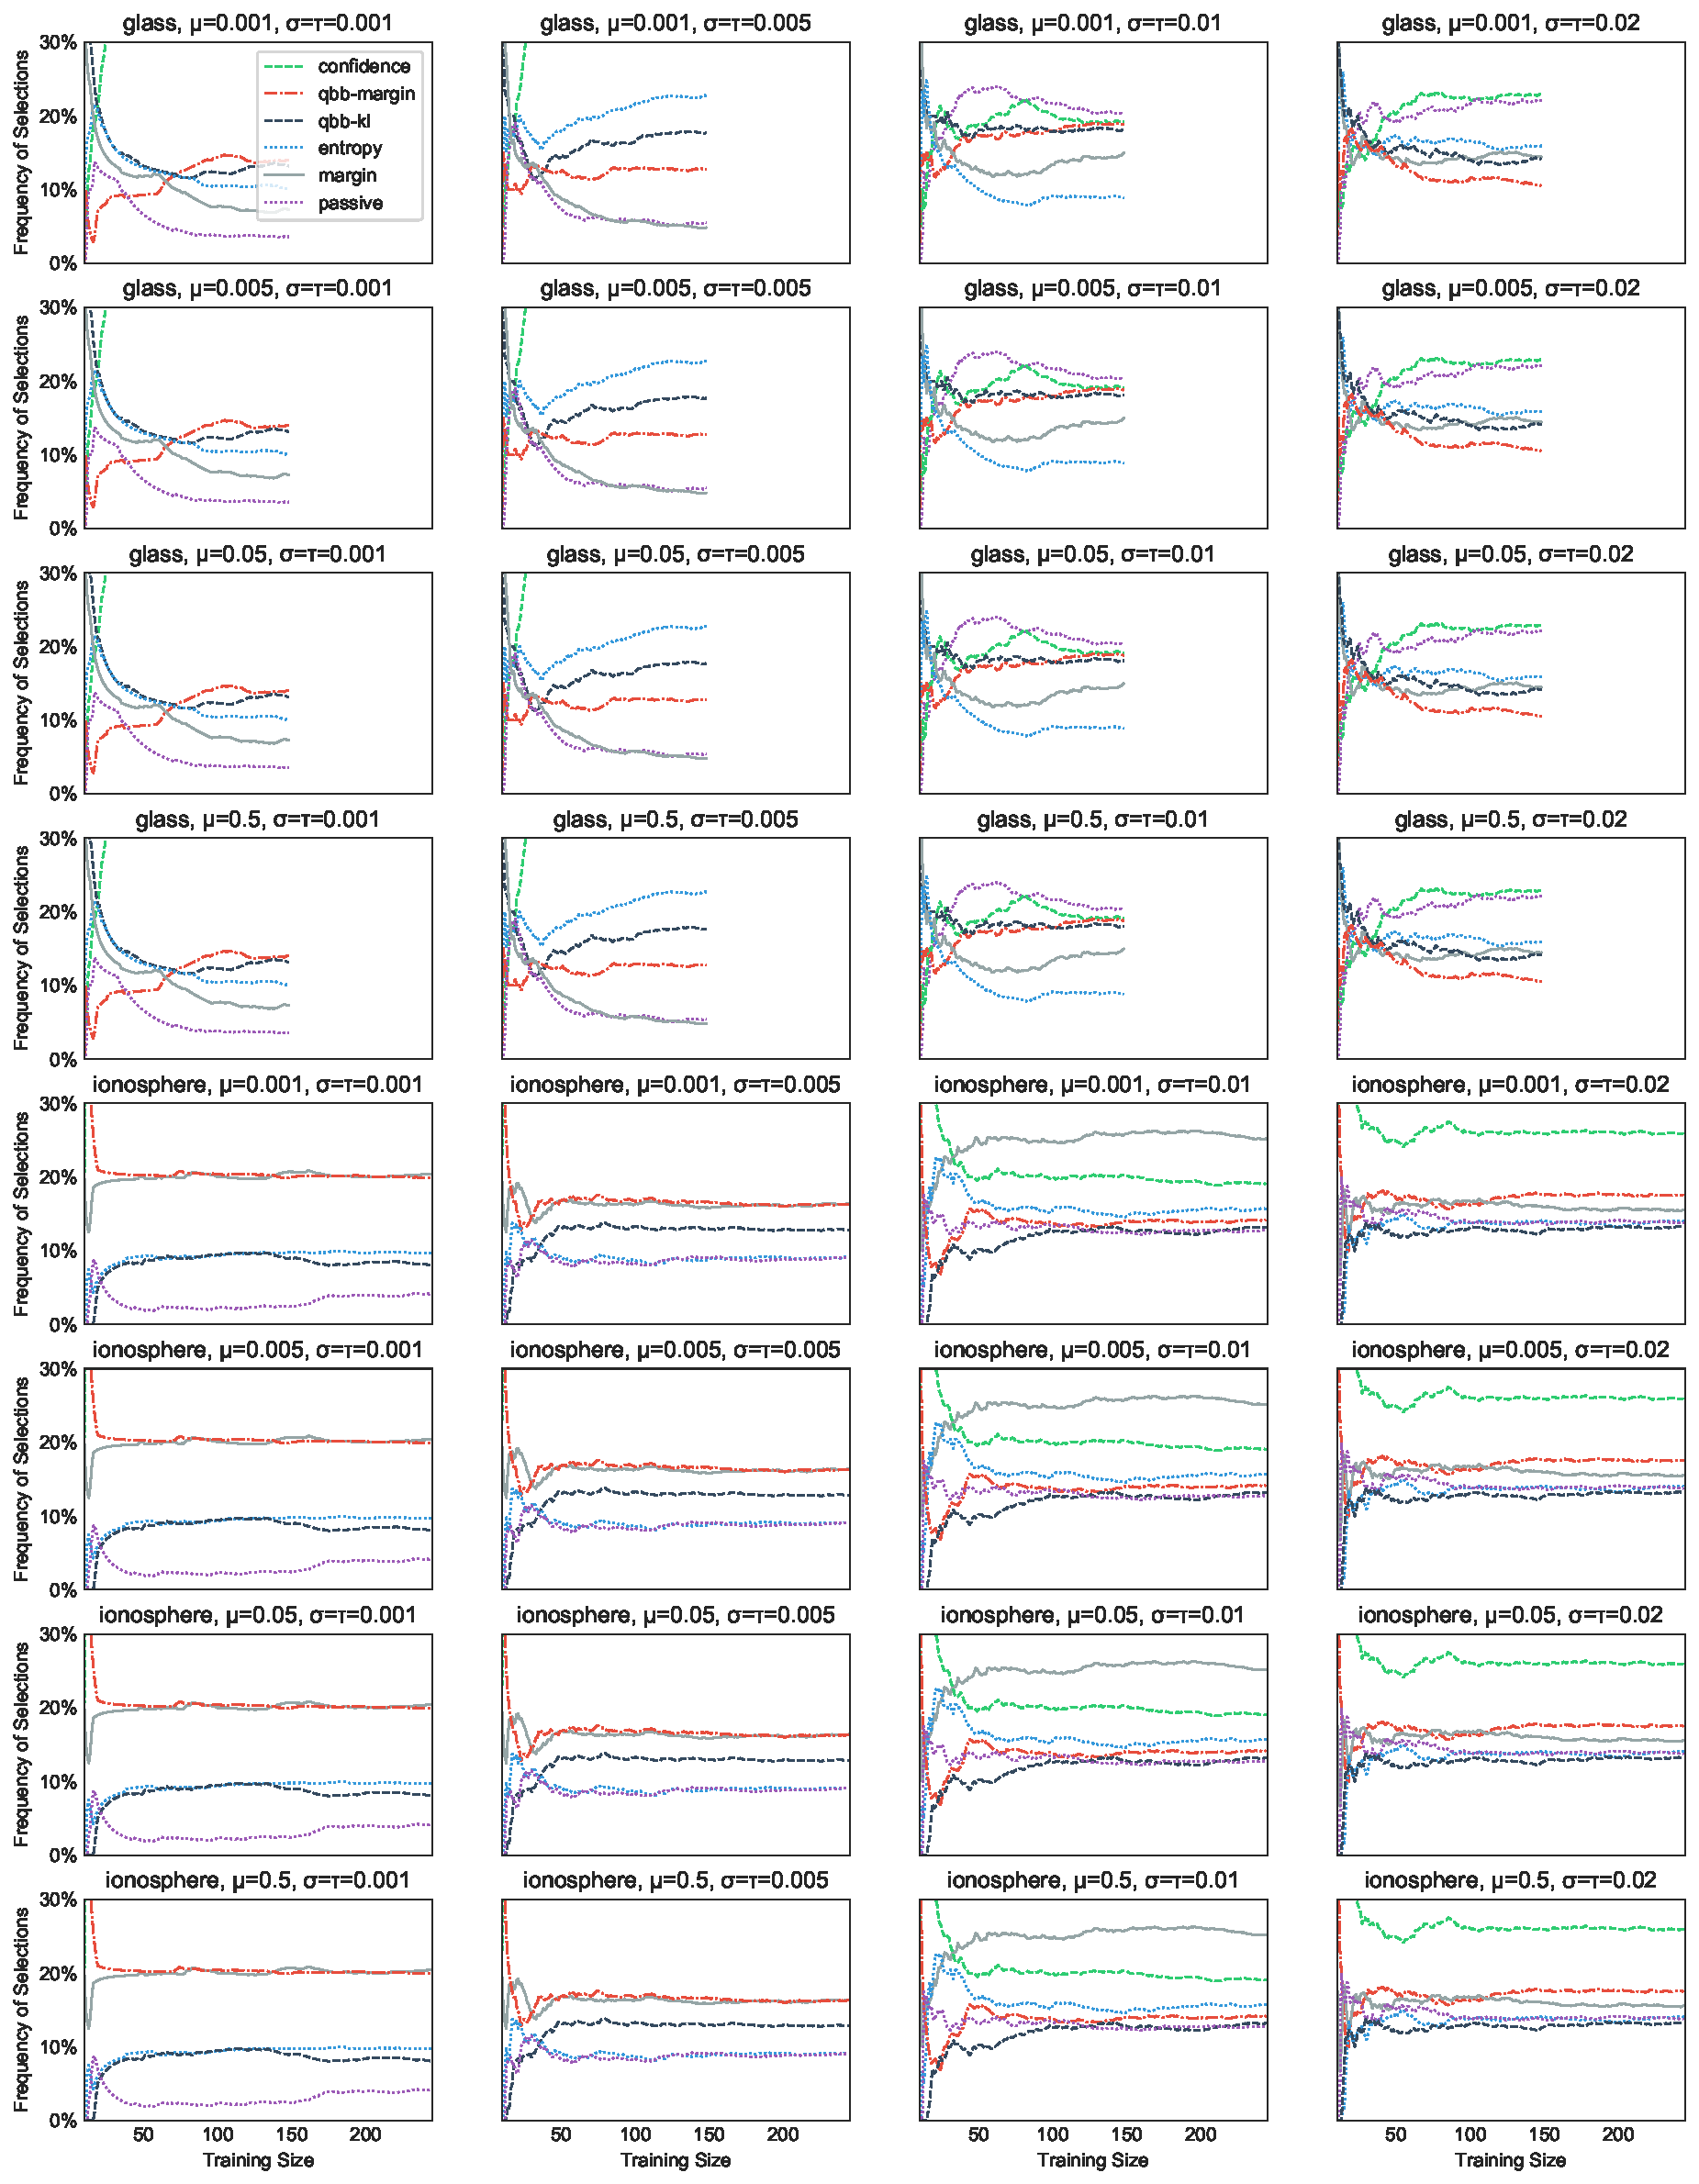
\includegraphics[width=\textwidth]{Fig11}
	\caption[Effect of hyperparameters on Thompson sampling on heuristic
	selection]{The effect of the initial values of the parameters in
	\textsc{thompson} on the heuristic selection frequencies. We test 16
	combinations of $\mu$, $\sigma^2$, and $\tau^2$ on the glass and ionosphere
	dataset. Which heuristics \textsc{thompson} picks seems to correlate with
	the heuristic performance. For example, in ionosphere, \textsc{passive}
	(the dotted purple line) and \textsc{qbb-kl} (the dashed dark blue line)
	tend to get picked less often than others.}
	\label{fig:selection-thompson-params}
\end{figure}

\begin{figure}[tbp]
	\centering
	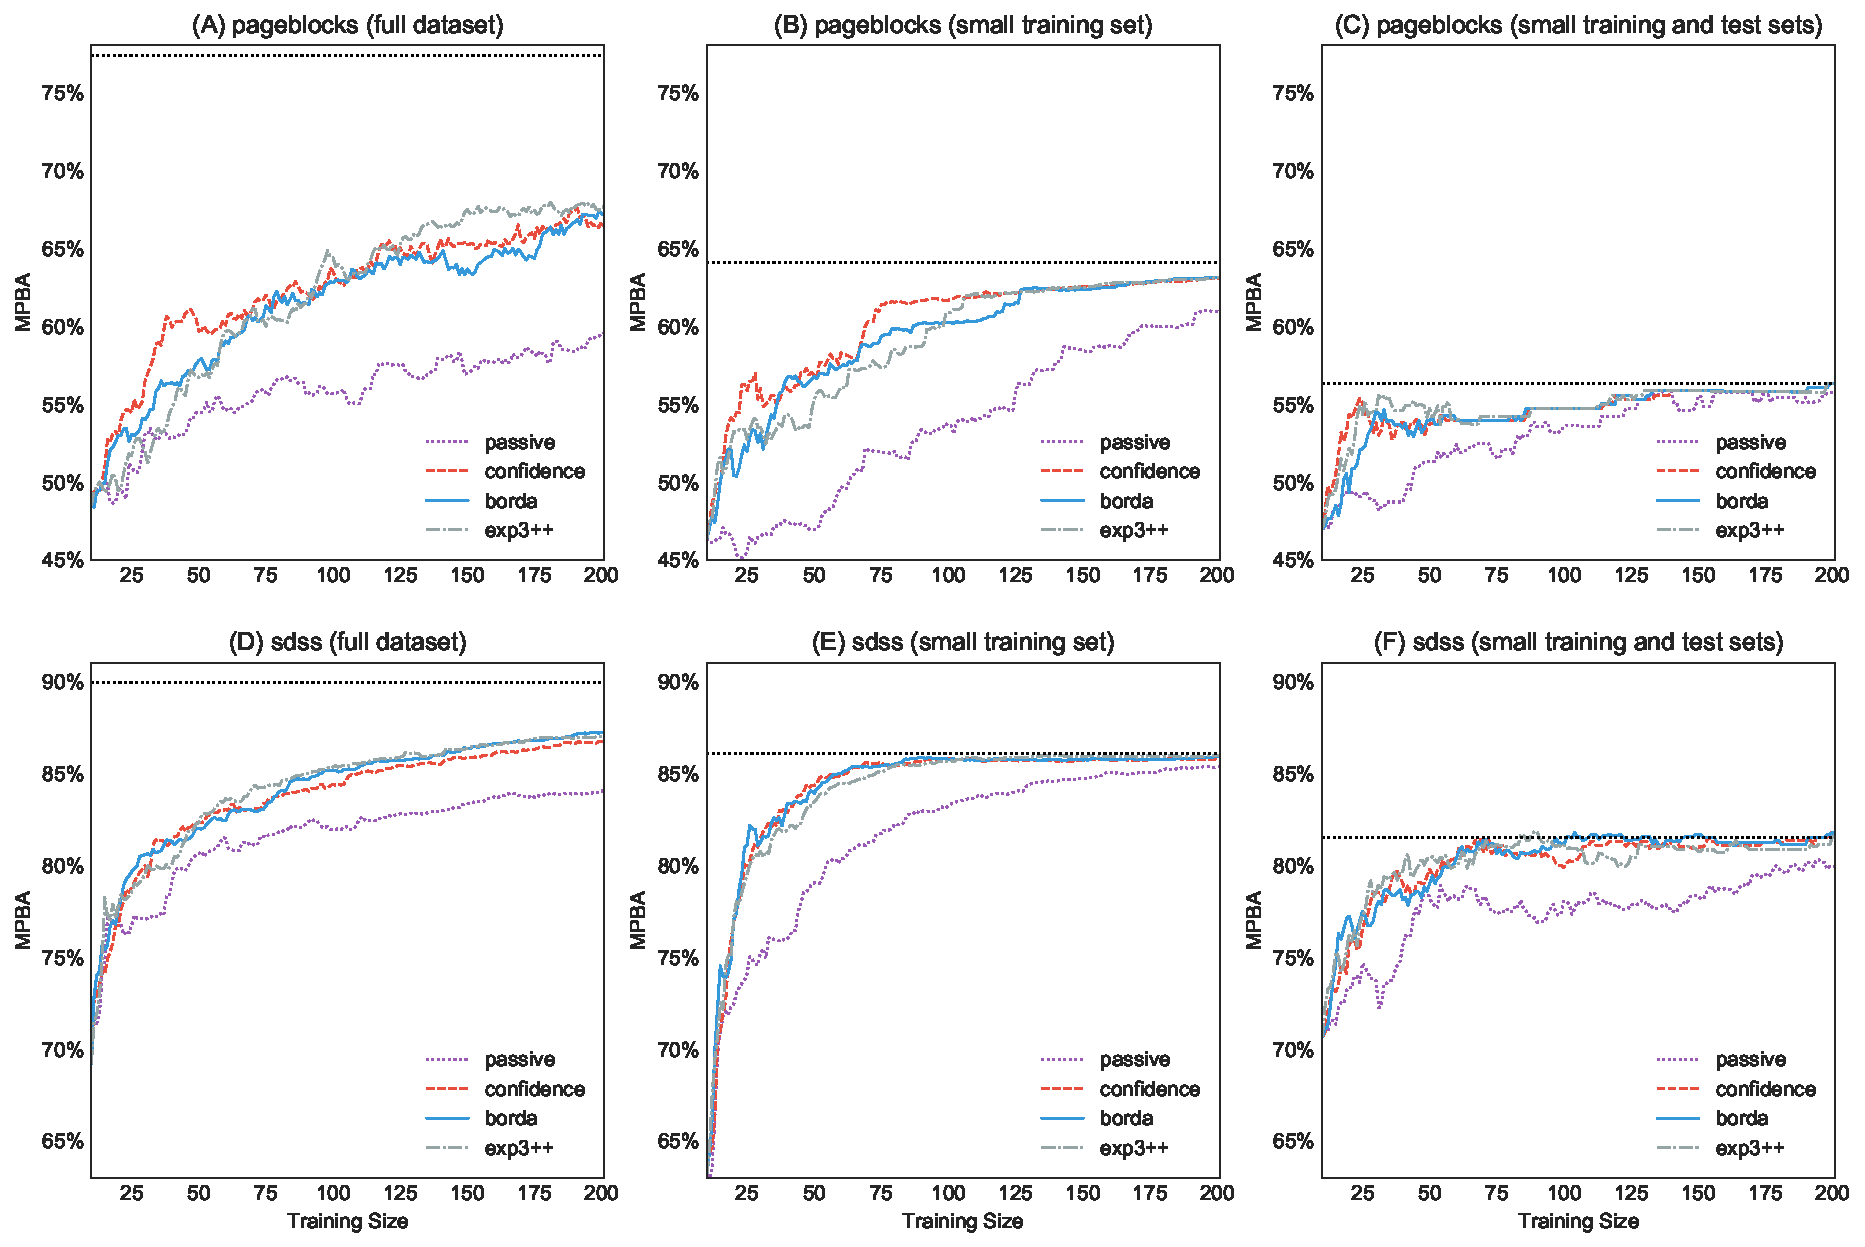
\includegraphics[width=\textwidth]{Fig12}
	\caption[Effect of the pool size]{Effect of the pool size on the learning
	curves. We pick two large datasets---pageblocks and sdss---to investigate
	how the size of the pool affects the performance. The leftmost figures (A
	and D) are the original learning curves from Figures
	\ref{fig:learning_curves-large}F and \ref{fig:learning_curves-large}J (we
	only show the first 200 examples so that all figures have the same scale).
	For the middle figures, we use the same test pool, but the unlabeled pool
	now only has a maximum of 300 candidates. Finally for the rightmost
	figures, the combined test pool and training pool have a size of 300.}
	\label{fig:learning-curves-pool-size}
\end{figure}

\section{Discussion}\label{sec:discussion}

The experimental results allow us to answer the following questions:

\begin{enumerate}
	\item \textbf{Can active learning beat passive learning?} Yes, active
	learning can perform much better than passive learning, especially when the
	unlabeled pool is large (e.g. sdss, miniboone, pageblock). When the
	unlabeled pool is small, the effect of active learning becomes less
	apparent, as there are now fewer candidates to choose from. This can be
	seen in Figure \ref{fig:learning-curves-pool-size}, where we show that
	artificially reducing the unlabeled pool results in a reduction in the
	final performance. At the same time, having a small test set also makes the
	gap between the active learning curve and the passive learning curve
	smaller (see the rightmost subplots of Figure
	\ref{fig:learning-curves-pool-size}). This further contributes to the
	poorer performance on the smaller datasets. In any case, when a dataset is
	small, we can label everything so active learning is usually not needed.

	\item \textbf{Can active learning degrade performance?} Yes, there is no
	guarantee that active learning will always beat passive learning. For
	example, \textsc{w-entropy} actually slows down the learning in the many
	datasets. However, this only happens with certain heuristics, like those
	using the information density weighting.

	\item \textbf{What is the best single active learning heuristic?} All of
	\textsc{confidence}, \textsc{margin}, \textsc{entropy}, and
	\textsc{qbb-margin} have a similar performance. However \textsc{confidence}
	is perhaps the simplest to compute and thus is a good default choice in
	practice.

	\item \textbf{What are the challenges in using bandit algorithms?}
	\begin{enumerate}
		\item Designing a good reward scheme is difficult. This paper uses the
		increase in the classifier performance as the reward. However this type
		of reward is non-stationary (i.e. it gets smaller after each step as
		learning saturates) and the rewards will thus eventually go to zero.
		\item In practice, we do not have a representative test set that can be
		used to compute the reward. As a workaround, \cite{hsu15} computed the
		reward on the training set and then used importance weighting to remove
		any potential bias. For this to work, we need to ensure that every
		training example and every active learning suggestion have a non-zero
		probability of being selected in each step.
		\item Finally, some bandit algorithms such as Thompson sampling
		assumes that the reward follows a certain distribution (e.g. Gaussian).
		However, this assumption is unrealistic.
	\end{enumerate}

	\item \textbf{What are the challenges in using rank aggregation
	algorithms?}
	\begin{enumerate}
		\item We need to compute the scores from all heuristics at every time
		step. This might not be feasible if there are too many heuristics or if
		we include heuristics that require a large amount of compute power
		(e.g. variance minimization).
		\item The Schulze method uses $O(n^2)$ space, where $n$ is the number
		of candidates. This might lead to memory issues if we need to rank
		a large number of candidates from the unlabeled pool.
		\item Before aggregating the rankings, we throw away the score
		magnitudes, which could cause a loss of information.
		\item Unlike bandit algorithms, all of the rank aggregators always give
		each heuristic an equal weight.
	\end{enumerate}

	\item \textbf{Which method should I use in practice to combine active
	learners?} Since there is no difference in performance between various
	combiners,  we recommend using a simple rank aggregator like Borda count or
	geometric mean if we do not want to select a heuristic a priori. Rank
	aggregators do not need a notion of a reward---we simply give all
	suggestions an equal weight when combining. Thus we neither need to a keep
	a separate test set, nor do we need to worry about designing a good reward
	scheme.
\end{enumerate}

Our investigation has a few limitations. Firstly, we empirically compare
algorithms that only work with single-label classification problems. Nowadays,
many problems require multi-label learning, in which each example is allowed to
be in more than one class. Our methods can be extended to work with multi-label
datasets with the following modifications. We first need a multi-label
classifier. This can be as simple as a collection of binary classifiers, each
of which produces the probability that an example belongs to a particular
class. For each class, we can use an active learning heuristic to assign a
score to each unlabeled example as before. However now we need to aggregate the
scores among the classes. As suggested by \cite{reyes18}, we can use any
aggregation method like Borda count to combine these scores. In effect, the
multi-label learning problem adds an extra layer of aggregation into the
pipeline.

Another limitation of our methods is that our active learning methods are
myopic. That is, in each iteration, we only pick one instance to give to a
human expert for labeling. In many practical applications like astronomy,
batch-mode active learning is preferred, as it is much more cost efficient to
obtain multiple labels simultaneously. One naive extension is to simply choose
the $m$ highest ranked objects using our current methods. However, it is
possible to have two unlabeled objects whose class membership we are currently
uncertain about, but because they have very similar feature vectors, labeling
only one of them would allow us to predict the label of the other one easily.
More sophisticated batch-mode active learning heuristics have been proposed,
for example by using cluster analysis \citep{xu07} or by maximizing the
diversity in a batch \citep{brinker03}. How to aggregate suggestions from these
heuristics is an interesting problem for future work.

\section{Conclusion}

In this paper we compared 16 active learning methods with passive learning.
Our three main findings are: active learning is better than passive learning;
combining active learners does not in general degrade the performance; and
social choice theory provides more practical algorithms than bandit theory
since we do not need to design a reward scheme.


\bibliography{active}

\pagebreak

\section*{Appendix A: Posterior Balanced Accuracy}


Most real-world datasets are unbalanced. In the SDSS dataset, for example,
there are 4.5 times as many galaxies as quasars. The problem of class imbalance
is even more severe in the pageblocks dataset, where one class makes up 90\% of
the data and the remaining four classes only make up 10\%. An easy fix is to
undersample the dominant class when creating the training and test sets. This,
of course, means that the size of these sets are limited by the size of the
minority class.

When we do not want to alter the underlying class distribution or when larger
training and test sets are desired, we need a performance measure that can
correct for the class imbalance.~\cite{brodersen10} show that the posterior
balanced accuracy distribution can overcome the bias in the binary case. We now
extend this idea to the multi-class setting.

Suppose we have $k$ classes. For each class $i$ between $1$ and $k$, there are
$N_i$ objects in the universe. Given a classifier, we can predict the label of
every object and compare our prediction with the true label. Let $G_i$ be the
number of objects in class $i$ that are correctly predicted.
Then we define the recall $A_i$ of class $i$ as\index{recall}
	\begin{align}
		A_i &= \frac{G_i}{N_i}
	\end{align}
The problem is that it is not feasible to get the actual values of $G_i$ and
$N_i$ since that would require us to obtain the true label of every object in
the universe. Thus we need a method to estimate these quantities when we only
have a sample. Initially we have no information about $G_i$ and $N_i$, so we
can assume that each $A_i$ follows a uniform prior distribution between 0 and
1. This is the same as a Beta distribution with shape parameters $\alpha =
\beta = 1$:
	\begin{align}
		A_i &\sim \Beta(1,1)
	\end{align}
The probability density function (PDF) of $A_i$ is then
    \begin{align}
        f_{A_i}(a) &= \frac{\Gamma(\alpha+\beta)}{\Gamma(\alpha)\Gamma(\beta)}\,
        a^{\alpha-1}(1-a)^{\beta-1} \label{eqn:prior} \\
        &\propto   a^{1-1}(1-a)^{1-1}  \notag
    \end{align}
where $\Gamma(\alpha)$ is the gamma function.

After we have trained the classifier, suppose we have a test set containing
$n_i$ objects in class $i$. Running the classifier on this test set is the same
as conducting $k$ binomial experiments, where, in the $i$th experiment, the
sample size is $n_i$ and the probability of success is simply $A_i$. Let $g_i$
be the number of correctly labeled objects belonging to class $i$ in the test
set. Then, conditional on the recall rate $A_i$, $g_i$ follows a binomial
distribution:
	\begin{align}
		(g_i \mid A_i) &\sim \Bin(n_i, A_i)
	\end{align}
The probability mass function of $(g_i \mid A_i = a)$ is thus
    \begin{align}
		p_{g_i \mid A_i}(g_i) &= \binom{n_i}{g_i} a^{g_i} (1 - a)^{n_i - g_i}
						  							\label{eqn:likelihood} \\
                              &\propto a^{g_i} (1 - a)^{n_i - g_i} \notag
    \end{align}
In the Bayesian \index{Bayesian} setting, Eq. ~\eqref{eqn:prior} is the prior
and Eq. \eqref{eqn:likelihood} is the likelihood. To get the posterior PDF, we
simply multiply the prior with the likelihood:
	\begin{align}
		f_{A_i \mid \bm{g}}(a)
		&\propto f_{A_i}(a) \times f_{g_i \mid A_i}(g_i) \\
		&\propto a^{1-1}(1-a)^{1-1} \times a^{g_i} (1 - a)^{n_i - g_i} \\
		&= a^{1 + g_i - 1}(1-a)^{1 + n_i - g_i - 1}
	\end{align}
Thus, with respect to the binomial likelihood function, the Beta distribution
is conjugate to itself. The posterior recall rate $A_i$ also follows a Beta
distribution, now with parameters
	\begin{align}
		(A_i \mid g_i) &\sim \Beta(1 + g_i, 1 + n_i - g_i)
	\end{align}
Our goal is to have a balanced accuracy rate, $A$, that puts an equal weight in
each class. One way to achieve this is to take the average of the individual
recalls:
	\begin{align}
		A &= \frac{1}{k} \sum_{i=1}^k A_i \\
		&= \frac{1}{k} A_T
	\end{align}
Here we have defined $A_T$ to be the sum of the individual recalls. We call $(A
\mid \bm{g})$ the posterior balanced accuracy, where $\bm{g} =(g_1,...,g_k)$.
Most of the time, we simply want to calculate its expected value:
	\begin{align}
		\E{A \given \bm{g}} &= \frac{1}{k} \, \E{A_T \given \bm{g}} \\
		&= \frac{1}{k} \int a \cdot f_{A_T \mid \bm{g}}(a) \, da
	\end{align}
Let us call this the mean posterior balanced accuracy (MPBA). Note that there
is no closed form solution for the PDF $f_{A_T \mid \bm{g}}(a)$. However
assuming that $A_T$ is a sum of $k$ independent Beta random variables, $f_{A_T
\mid \bm{g}}(a)$ can be approximated by numerically convolving $k$ Beta
distributions. The independence assumption is reasonable here, since there
should be little to no correlation between the individual recall rates. For
example, knowing that a classifier is really good at recognizing stars does not
tell us much about how well that classifier can recognize galaxies.

Having the knowledge of $f_{A \mid \bm{g}}(a)$ will allow us to make violin
plots, construct confidence intervals and do hypothesis tests. To get an
expression for this, let us first rewrite the cumulative distribution function
(CDF) as
	\begin{align}
		F_{A\mid \bm{g}}(a) &= \Prob{A \leq a \mid \bm{g}} \\
		&= \Prob[\Big]{\frac{1}{k} A_T \leq a \given \bm{g}} \\
		&= \Prob{A_T \leq ka \given \bm{g}} \\
		&= F_{A_T \mid \bm{g}}(ka) \IEEEyesnumber \label{eqn:CDF}
	\end{align}
Differentiating \eqref{eqn:CDF} with respect to $a$, we obtain the PDF of $(A \mid \bm{g})$:
	\begin{align}
		f_{A \mid \bm{g}}(a) &= \frac{\partial}{\partial a} F_{A \mid \bm{g}}(ka) \\
		&= \frac{\partial}{\partial a} (ka) \cdot \frac{\partial}{\partial ka}
			F_{A_T \mid \bm{g}}(ka) \\
		&= k \cdot f_{A_T \mid \bm{g}}(ka)
	\end{align}
A Python implementation for the posterior balanced accuracy can be found
on our GitHub repository\footnote{\url{https://github.com/chengsoonong/mclass-sky}}.
\end{document}
